\documentclass[10pt]{article}
\usepackage{tmlr}
% For camera-ready (accepted): \usepackage[accepted]{tmlr}
% For preprint/arXiv: \usepackage[preprint]{tmlr}

% Optional math commands from Deep Learning book notation
\input{math_commands.tex}

%%% Packages ported from IEEE TAI submission %%%
\usepackage[colorlinks,urlcolor=blue,linkcolor=blue,citecolor=blue]{hyperref}
\usepackage{url}
\usepackage{graphicx}
\usepackage{amsmath}
\usepackage{amssymb}
\usepackage{amsfonts}
\usepackage{mathtools}
\usepackage{mathrsfs}
\usepackage{algorithm}
\usepackage{algpseudocode}
\usepackage{multirow}
\usepackage{makecell}
\usepackage{booktabs}
\usepackage{colortbl}
\usepackage{xcolor}
\usepackage{float}
\usepackage{placeins}
\usepackage{adjustbox}
\usepackage{cancel}
\usepackage{pdflscape}
\usepackage{pifont}
\usepackage{soul}
\usepackage{array}
\usepackage{subcaption}



% Custom commands
\newcommand{\cmark}{\ding{51}}
\newcommand{\xmark}{\ding{55}}
\definecolor{bestgreen}{RGB}{144, 238, 144}
\definecolor{secondblue}{RGB}{173, 216, 230}
\newcommand{\best}[1]{\cellcolor{bestgreen}#1}
\newcommand{\second}[1]{\cellcolor{secondblue}#1}
\setlength{\fboxsep}{1pt}

% Theorem environments
\newtheorem{theorem}{Theorem}
\newtheorem{lemma}{Lemma}

\renewcommand{\topfraction}{0.85}
\renewcommand{\bottomfraction}{0.85}
\renewcommand{\textfraction}{0.10}
\renewcommand{\floatpagefraction}{0.75}
\setcounter{topnumber}{3}
\setcounter{bottomnumber}{3}
\setcounter{totalnumber}{5}

%%% Paper metadata (review version: authors hidden) %%%
\title{BID-LoRA: A Parameter-Efficient Framework for Continual Learning and Unlearning}

% Authors must not appear in the submitted version.
% Non-anonymous submissions will be rejected without review.
% \author{\name Jagadeesh~Rachapudi \email s23096@students.iitmandi.ac.in \\
%       \addr Indian Institute of Technology Mandi, India
%       \AND
%       \name Ritali~Vatsi \email d23059@students.iitmandi.ac.in \\
%       \addr Indian Institute of Technology Mandi, India
%       \AND
%       \name Praful~Hambarde \email praful@iitmandi.ac.in \\
%       \addr Indian Institute of Technology Mandi, India
%       \AND
%       \name Amit~Shukla \email amitshukla@iitmandi.ac.in \\
%       \addr Indian Institute of Technology Mandi, India}

% \def\month{MM}
% \def\year{YYYY}
% \def\openreview{\url{https://openreview.net/forum?id=XXXX}}

\begin{document}

\maketitle

\begin{abstract}
\label{abstract}
Recent advances in deep learning underscore the need for systems that can not only acquire new knowledge through Continual Learning (CL) but also remove outdated, sensitive, or private information through Machine Unlearning (MU). However, while CL methods are well-developed, MU techniques remain in early stages, creating a critical gap for unified frameworks that depend on both capabilities. We find that naively combining existing CL and MU approaches results in \textit{knowledge leakage} a gradual degradation of foundational knowledge across repeated adaptation cycles. To address this, we formalize Continual Learning Unlearning (CLU) as a unified paradigm with three key goals: (i) precise deletion of unwanted knowledge, (ii) efficient integration of new knowledge while preserving prior information, and (iii) minimizing knowledge leakage across cycles. We propose Bi-Directional Low-Rank Adaptation (BID-LoRA), a novel framework featuring three dedicated adapter pathways-retain, new, and unlearn-applied to attention layers, combined with escape unlearning that pushes forget-class embeddings to positions maximally distant from retained knowledge, updating only $\approx$5\% of parameters. Experiments on CIFAR-100 show that BID-LoRA outperforms CLU baselines across multiple adaptation cycles. We further evaluate on CASIA-Face100, a curated face recognition subset, demonstrating practical applicability to real-world identity management systems where new users must be enrolled and withdrawn users removed.
\end{abstract}

% \def\abstractname{Impact Statement}
% \begin{abstract}
% This work advances responsible AI by enabling models to selectively forget sensitive data while continuously learning critical for GDPR/CCPA compliance in identity management. BID-LoRA's parameter efficiency (5\% updates) trimmed for continual adaptations for resource-constrained deployments, while escape unlearning provides verifiable privacy protection against membership inference attacks.
% \end{abstract}

% \begin{IEEEkeywords}
% Continual Learning, Machine Unlearning, LoRA, Parameter-Efficient Fine-Tuning
% \end{IEEEkeywords}
\section{Introduction}
\label{1.0}


Recent developments in AI have triggered a new shift in deep learning models~\cite{kaplan2020scaling}. Future intelligent systems are expected to follow a dual paradigm: learn new knowledge, and remove specific knowledge. This capability is called Continual Learning and Unlearning (CLU) \cite{chatterjee2024unified,liu2022continual}, also termed continual adaptation. This capability becomes essential when data distributions shift over time, whether due to policy changes, task modifications, or market trends. Regardless of the underlying cause, the model's knowledge base must be updated accordingly. Fig~\ref{fig:1} illustrates CLU system as new data replaces unwanted data. This requires simultaneous systems for both learning and unlearning.

Since CLU combines Continual Learning (CL) and Machine Unlearning (MU), we establish each component's foundation. CL is the process of acquiring new knowledge~\cite{kirkpatrick2017overcoming,buzzega2020dark,caccia2021new,douillard2022dytox,cotogni2025exemplar,mohamed2023d3former} from unseen data while retaining performance on existing tasks, widely studied in machine learning. Application tasks include mixed-task scenarios, out of distribution tasks, among others. While CL focuses on knowledge acquisition, MU addresses selective knowledge removal, an emerging field~\cite{kurmanji2023towards,zhao2024continual,cha2024learning,fan2023salun,tarun2023fast}. Targets for unwanted knowledge removal include privacy-related data, regulatory removal by government orders such as General Data Protection Regulation (GDPR) and California Consumer Privacy Act (CCPA)~\cite{goldman2020introduction,data2018general}, and hate speech, among others.

\begin{figure}[!htbp]
    \centering
    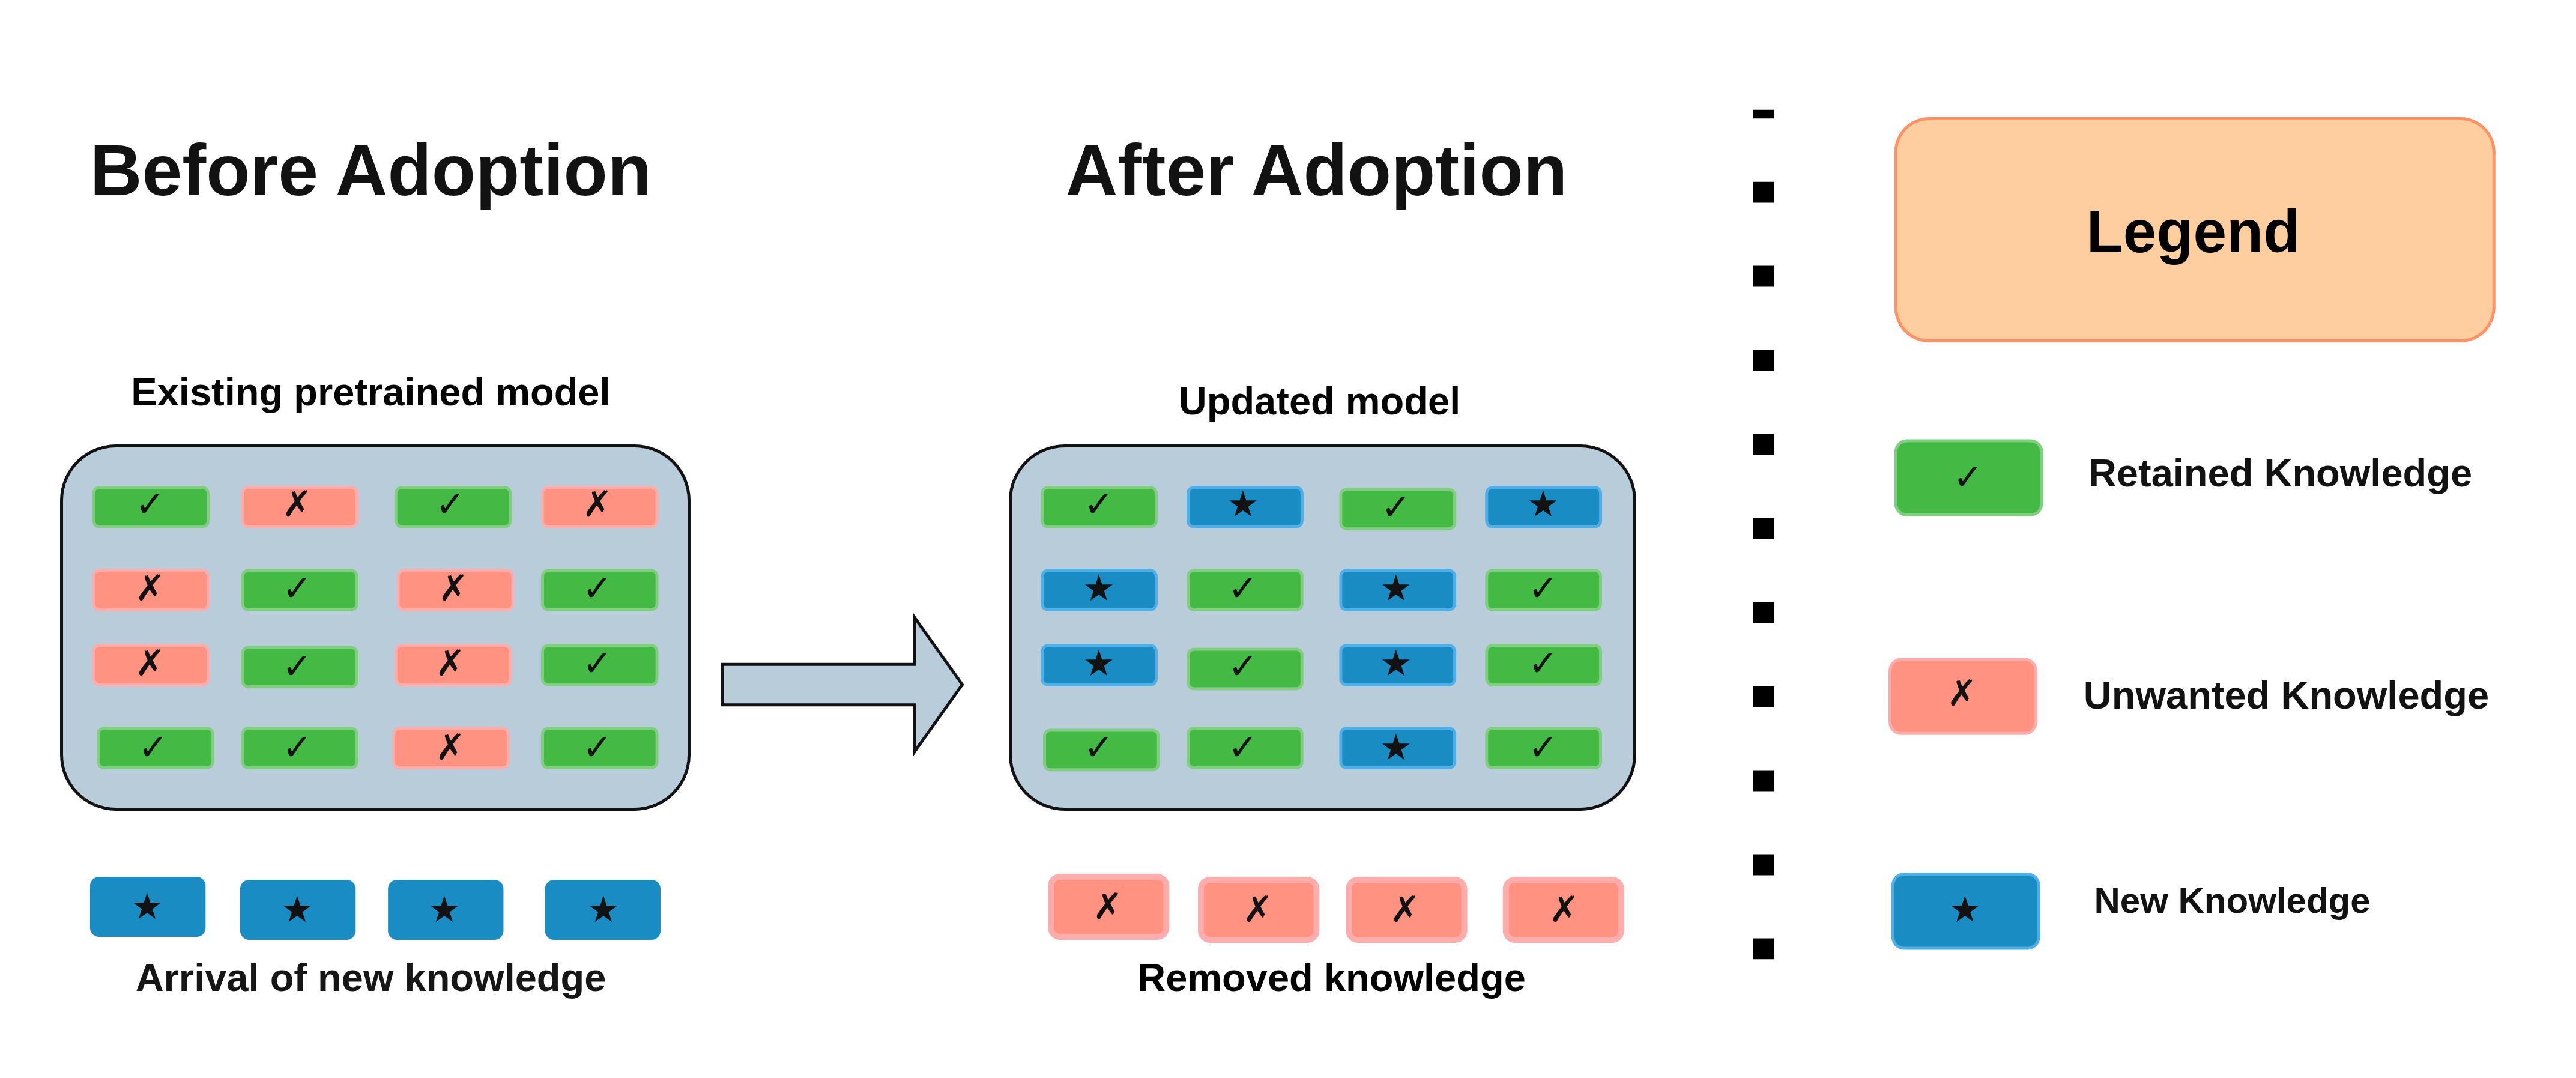
\includegraphics[width=0.75\textwidth]{images/overview.drawio.png}
    \caption{Overview of CLU. The CLU system removes unwanted knowledge (\textcolor{red}{red}), retains prior knowledge (\textcolor[HTML]{006400}{green}), and integrates new knowledge (\textcolor{blue}{blue}).}
    \label{fig:1}
\end{figure}


There is an intrinsic connection between MU and CL in which one adds knowledge and other removes knowledge, both retaining existing knowledge. Can we combine both for simultaneous learning and unlearning? Such a framework would enable access control, surveillance, personalized education, and content moderation. Can continual learning alone solve this? No-without removing unwanted knowledge over time, it accumulates and causes knowledge drift   degrading model performance and creating bias toward unwanted information, making unlearning essential.

Despite CLU's importance, a research gap exists due to maturity imbalance. CL is well-established, while Machine Unlearning remains developmental. This disparity leaves unified CLU frameworks largely unexplored. CLU applications demand parameter-efficient solutions. CLU systems continuously adapt as data arrives and require removal. Full retraining becomes computationally infeasible, making parameter-efficient approaches essential. However, combining CL and MU introduces knowledge leakage-repeated learning-unlearning cycles cause models to gradually lose foundational knowledge. Unlike catastrophic forgetting, knowledge leakage is a slow degradation of original capabilities across adaptation cycles; further analysis is provided in Section~\ref{8.2}. This challenge is critical because real-world systems face continuous requests: employees join and leave organizations, regulations evolve, and user preferences shift constantly. Such systems with minimal knowledge leakage would enable critical applications: language models, medical systems, recommendation engines, and autonomous vehicles. Face recognition presents the most urgent CLU need due to privacy challenges.


Face recognition systems are critical CLU applications as personnel frequently join and leave organizations. Since facial data is highly sensitive private information, protecting it from misuse through model inversion techniques~\cite{fredrikson2015model,zhu2019deep,zhang2020secret} becomes essential to safeguard privacy rights mandated by GDPR and CCPA~\cite{goldman2020introduction,data2018general}. Face recognition thus provides a natural testbed for CLU applications, presenting an urgent challenge that demands immediate attention given the escalating privacy threats and regulatory requirements. Designing such an ideal CLU system presents three core challenges. First, achieving continual learning while avoiding catastrophic forgetting. Second, implementing selective machine unlearning. Finally, maintaining knowledge stability and minimizing knowledge leakage across repeated cycles. 

To address these challenges, we propose Bi-Directional LoRA (BID-LoRA), a parameter-efficient solution to CLU problems that minimizes knowledge leakage. BID-LoRA leverages LoRA's inherent parameter efficiency, fine-tuning only attention layers in transformer blocks and classification heads~\cite{houlsby2019parameter,hu2022lora,li2021prefix,geva2020transformer} as fine-tuning fewer parameters has been shown effective~\cite{mallya2018packnet,mallya2018piggyback,wang2022learning,zhang2022continual} in knowledge manipulation. To reduce catastrophic forgetting~\cite{kirkpatrick2017overcoming} and minimize knowledge leakage, we employ the replay mechanism. This approach is similar to performing minimally invasive surgery on a model rather than major surgery. BID-LoRA is simple, parameter-efficient, data-efficient, and suitable for large models. We conduct extensive experiments across classification and face recognition tasks, demonstrating broad applicability. Our contributions are summarized as follows:
\label{contributions}
\begin{itemize}
    \item We formally define the Continual Learning-Unlearning (CLU) problem and demonstrate that naively combining existing CL and MU approaches leads to significant knowledge leakage, where foundational knowledge degrades across repeated adaptation cycles.
    
    \item We propose BID-LoRA, a parameter-efficient framework featuring three-pathway separation that isolates retained, forgotten, and newly learned knowledge. This architecture prevents interference between competing objectives while updating only $\approx$5\% of model parameters.
    
    \item We introduce escape unlearning, which computes optimal embedding locations that are maximally distant from retained class centroids, pushing forget-class representations to positions that are both hard to recover and non-interfering with retained knowledge.
    
    \item We establish the first generalizable CLU benchmark through comprehensive experiments on CIFAR-100 and CASIA-Face100, employing a novel sliding window evaluation protocol with progressive 10-class forget-retain-learn cycles that systematically tests long-term adaptation stability.
    
    \item We demonstrate BID-LoRA's practical applicability to face recognition and identity management systems, where privacy-driven unlearning (e.g., GDPR compliance) must coexist with incremental enrollment of new users.
\end{itemize}
\section{Related work}
\label{2}
\subsection{Continual Learning}
\label{2.1}
Continual Learning (CL) aims to train models sequentially on evolving tasks while retaining prior knowledge. In the CL setting, new classes arrive without access to old data, often leading to catastrophic forgetting. To address this, several strategies have emerged.  

Kirkpatrick \textit{et al.} ~\cite{kirkpatrick2017overcoming} introduced Elastic Weight Consolidation (EWC), an early exemplar-free approach that adds a Fisher-based quadratic penalty to protect parameters critical for past tasks. Buzzega \textit{et al.} ~\cite{buzzega2020dark} proposed Dark Experience Replay++ (DER++), combining rehearsal with distillation by storing both samples and logits to stabilize decision boundaries. Caccia \textit{et al.} ~\cite{caccia2021new} developed ER-ACE and ER-AML where cross-entropy is applied asymmetrically, isolating new-class updates while replay consolidates all classes. Douillard \textit{et al.} ~\cite{douillard2022dytox} presented DyTox, a transformer-based method using task-specific tokens and a replay buffer to scale across tasks without task IDs. Cotogni \textit{ et al.} ~\cite{cotogni2025exemplar} introduced GCAB, which employs gated class attention and feature drift compensation for exemplar-free ViT learning. Finally, Mohamed \textit{et al.} ~\cite{mohamed2023d3former} proposed D3Former, which debiases logits and preserves attention maps to balance performance across old and new classes.
  
 
\subsection{Machine Unlearning}
\label{2.2}
Machine Unlearning (MU) has seen significant advancements, focusing on methods that effectively balance the removal of data influence and the preservation of retained knowledge. Kurmanji \textit{et al.} \cite{kurmanji2023towards} tackled the problem of unlearning by pushing the forget distribution toward a uniform distribution, while ensuring that the retain distribution follows the normal loss function. This approach ensures that models forget the target data without significantly compromising performance on the remaining data. Zhao \textit{ et al.} \cite{zhao2024continual} addressed the issue of continual forgetting in the context of continual learning by utilizing GS-LoRA, which targets the FFN modules with a group sparsity regularizer. Cha \textit{et al.} \cite{cha2024learning} introduced adversarial examples as a technique to ensure a cleaner and more robust removal of forget data. By generating adversarial examples, the model is encouraged to misclassify the forget data, making it harder for the model to remember or retain the forgotten samples. Fan \textit{et al.} \cite{fan2023salun} proposed a novel method that computes the weight saliency matrix for data to be forgotten. By identifying the most relevant weights for the forgotten samples, the model updates only those weights, which helps to avoid catastrophic forgetting and ensures that the model retains critical information from the retained data. Tarun \textit{et al.}~\cite{tarun2023fast} proposed a method that corrupts the knowledge to be forgotten by using noise and then performs repair work to maintain the retained knowledge. Panda \textit{et al.}~\cite{panda2024fast} proposed a weak unlearning approach for black-box GANs that filters undesired outputs by computing projection similarity between sampled latent vectors and a learned representation of unwanted features in the latent space. Wang \textit{et al.}~\cite{wang2025malicious} proposed MCC-Fed, which detects malicious clients via Euclidean distance-based deviation analysis and employs a Lipschitz-inspired contribution-aware metric as a regularization term to precisely unlearn their negative influence without requiring auxiliary datasets.

\subsection{Parameter-Efficient Fine-Tuning}
\label{2.3}
Fine-tuning large pretrained models such as vision and language models on downstream tasks has become a dominant paradigm in modern deep learning. Parameter-efficient fine-tuning techniques are widely adopted, as they substantially reduce trainable parameters without significant performance degradation. Addition-based approaches \cite{liu2024gpt} introduce new trainable components while freezing the original model; other works include \cite{houlsby2019parameter,li2021prefix}. Freezing-based techniques \cite{lee2019would} represent another approach, selectively updating only specific parameters or layers while keeping the rest frozen. Parameter factorization methods \cite{chavan2023one,valipour2022dylora} form the third category, decomposing weight updates into low-rank matrices to achieve efficiency. Among these, Low-Rank Adaptation (LoRA)~\cite{hu2022lora} has emerged as particularly effective, decomposing weight updates into low-rank matrices that can be efficiently trained and merged. Our work builds upon LoRA's foundation to address the unique challenges of continual learning-unlearning.

\subsection{Continual Learning-Unlearning (CLU)}
\label{2.4}
The existing CLU works, such as Shibata \textit{et al.} ~\cite{shibata2021learning}, Liu \textit{et al.}  ~\cite{liu2022continual}, Chatterjee \textit{et al.} ~\cite{chatterjee2024unified}, and Huang \textit{et al.} ~\cite{huang2025unified}, integrate CL and MU, providing theoretical foundations for adaptive knowledge management. While this field has gained attention, existing approaches still face significant design and efficiency challenges.  

Shibata \textit{et al.} ~\cite{shibata2021learning} first explored a CLU-like system using mnemonic codes, enabling selective forgetting by discarding class-specific codes and new learning by embedding fresh ones. However, this method requires retraining from scratch with mnemonic embeddings, is incompatible with pre-trained models, and doubles computational cost. Liu \textit{et al.} ~\cite{liu2022continual} proposed CLPU-DER++, which achieves exact unlearning via isolated temporary networks that can be deleted while retaining a permanent model. It guarantees privacy and supports selective forgetting without original data. Yet, it demands retraining from scratch, incurs exponential storage overhead with multiple tasks, and cannot revise permanent knowledge. Chatterjee \textit{et al.} ~\cite{chatterjee2024unified} introduced UniCLUN, a dual-teacher distillation framework with one CL teacher, one UL teacher, and a student model. It is the first unified CL–UL approach, handling mixed learning–forgetting sequences adaptively. Nevertheless, it incurs parameter overhead, requires heavy computation, and depends on replay buffers that raise privacy risks. Adhikari \textit{et al.} ~\cite{adhikari2025unlearning} proposed UnCLe, a hypernetwork-based framework that generates task-specific parameters conditioned on task embeddings, enabling data-free unlearning by aligning forget-task parameters with Gaussian noise. However, it supports only task-level unlearning and cannot be directly applied to pretrained models like DeiT, as it requires training a hypernetwork to generate entire model parameters from scratch rather than fine-tuning existing weights. More recently, Huang \textit{et al.} ~\cite{huang2025unified} proposed a gradient-based, task-agnostic CLU framework optimized via KL divergence, aiming for efficiency and adaptability. However, it requires computing online Hessian approximations through costly inner-loop optimization, lacks support for pretrained vision transformers, and has only been validated on models trained from scratch rather than leveraging existing foundation models.

Despite these contributions, none of the above methods are resource-friendly: most update nearly all parameters, making them inefficient for large-scale pre-trained models. Moreover, they have only been tested on limited scenarios involving a few additions and deletions, raising questions about their claims of `continual' operation. In contrast, our BID-LoRA is explicitly designed to be parameter-efficient, resource-conscious, and validated across long sequences of CLU requests, demonstrating genuine continual adaptability at scale.
\section{Problem Formulation}
\label{3}
\subsection{Problem Setting}
We introduce a novel problem setting called Continual Learning Unlearning (CLU) also known as Continual Adaptation or simply Adaptations, a framework for dynamically modifying model knowledge defined as learned class mappings encoded in parameters. This setting brings together two complementary goals: (i) selectively removing specific targeted knowledge (machine unlearning) and (ii) acquiring new targeted knowledge for existing pre-trained models (continual learning), all while maintaining performance on the remaining knowledge in a continual form. To develop a solution for this problem, we first present the most basic case, in which only one adaptation task is performed, and then expand this formulation to the continuous scenario, which includes a series of adaptation activities.

Let $\mathcal{M}$ be a model pre-trained on the dataset $D$. We regard $\mathcal{M}$ as a mapping function $f_\mathcal{M} : \mathcal{X}_D \rightarrow \mathcal{Y}_D$, where $\mathcal{X}_D$ and $\mathcal{Y}_D$ denote the input and output spaces associated with $D$, respectively. Our objective is to selectively discard certain knowledge while adding new knowledge and retaining the rest. We assume $D_f$ be the dataset to be forgotten, $D^\text{\textit{full}}_r$ the dataset to be retained, and $D_{\text{new}}$ the new dataset to be learned, satisfying $D = D^\text{\textit{full}}_r \cup D_f$, $D^\text{\textit{full}}_r \cap D_f = \emptyset$, and $D_{\text{new}} \cap D = \emptyset$.

In practice, storing the full retain set is prohibited under General Data Protection Regulation (GDPR) and California Consumer Privacy Act (CCPA) regulations for privacy-sensitive data, while for non-private data, retraining remains computationally expensive due to large-scale models and datasets. We therefore maintain a small replay buffer $D_r \subset D^\text{\textit{full}}_r$ such that $|D_r| \ll |D^\text{\textit{full}}_r|$ (at least 10\% of $|D^\text{\textit{full}}_r|$), here $D^\text{\textit{full}}_r$ represents full retaining data \footnote{From this point, $D_r$ denotes the experience replay buffer unless specified.}. The consequences of insufficient or absent buffer size are discussed in detail in Section~\ref{8.1}.


Before adaptation, $\mathcal{M}$ performs well on $D_r$ and $D_f$ but poorly on $D_{\text{new}}$, i.e.,
{\small
\begin{equation}
f_{\mathcal{M}} :
\mathcal{X}_{D_f} \rightarrow \mathcal{Y}_{D_f} \; ; \;
\mathcal{X}_{D_r} \rightarrow \mathcal{Y}_{D_r} \; ; \;
\mathcal{X}_{D_{\text{new}}} \cancel{\rightarrow} \mathcal{Y}_{D_{\text{new}}}.
\label{eq:1}
\end{equation}
}

Let the adaptation algorithm be $\mathcal{F}$ for more details please refer Section \ref{4} which modifies the model $\mathcal{M}$ to obtain $\mathcal{M'}$ by using $\mathcal{F}$ such that $\mathcal{M}' = \mathcal{F}(\mathcal{M}, D_f, D_r, D_{\text{new}})$ such that $\mathcal{M'}$ holds a new mapping relationship $f_{\mathcal{M}'}$ as 

{\small
\begin{equation}
f_{\mathcal{M'}} :
\mathcal{X}_{D_f} \cancel{\rightarrow} \mathcal{Y}_{D_f} \; ; \;
\mathcal{X}_{D_r} \rightarrow \mathcal{Y}_{D_r} \; ; \;
\mathcal{X}_{D_{\text{new}}} \rightarrow \mathcal{Y}_{D_{\text{new}}}.
\label{eq:2}
\end{equation}
}
Here, \( \cancel{\rightarrow} \) denotes that the mapping no longer holds (i.e., the model has forgotten the corresponding mapping), while \( \rightarrow \) indicates that the mapping still holds. 

We now extend this problem to the continual setting, where the model is required to sequentially adopt new knowledge, involving both unlearning and learning across tasks $T$. These tasks may be triggered by requests from the user, the owner, or both. Here, $t$ is an index representing the task number, ranging from $0, 1, 2, \ldots, t, \ldots, T$. let $D_r^\text{(t)}$ be the data to be retained, $D_{f}^\text{(t)}$ be the data to be forgotten and $D_\text{new}^\text{(t)}$ be the data to be learned at $t_\text{th}$ step respectively.

The algorithm $\mathcal{F}$ is applied as:
\[
    \mathcal{M}^\text{(t)} = \mathcal{F}(\mathcal{M^\text{{(t - 1)}}}, D_{f}^\text{(t)}, D_{r}^\text{(t)}, D_{\text{new}}^\text{(t)})
\]

The adaptation algorithm $\mathcal{F}$ takes the previous-step model $\mathcal{M^\text{{(t - 1})}}$ along with the datasets 
$D_{r}^\text{(t)}$, $D_{f}^\text{(t)}$, and $D_{\text{new}}^\text{(t)}$ to produce the updated model $\mathcal{M^\text{(t)}}$. Thus, $\mathcal{F}$ handles adaptation requests sequentially, starting from $\mathcal{M}$ and generating  a sequence of models $\mathcal{M^\text{(1)}}, \; \mathcal{M^\text{(2)}}, \; \mathcal{M^\text{(3)}}, \; \ldots, \; \mathcal{M^\text{(t)}}, \; \ldots, \; \mathcal{M^\text{(T)}}$,  where $\mathcal{M^\text{(t)}}$ represents the modified model after the $t$-th adaptation task.

After step $t$, the adapted model $\mathcal{M}^{(t)}$ must satisfy:

\begin{subequations}
\label{Eq:3}
\begin{align}
    f_{\mathcal{M}^{(t)}} &: \mathcal{X}_{D_{f}^{(i)}} \cancel{\rightarrow} \mathcal{Y}_{D_{f}^{(i)}}, \quad \forall \, i \leq t \label{Eq:3a} \\
    f_{\mathcal{M}^{(t)}} &: \mathcal{X}_{D_{r}^{(t)}} \rightarrow \mathcal{Y}_{D_{r}^{(t)}} \label{Eq:3b} \\
    f_{\mathcal{M}^{(t)}} &: \mathcal{X}_{D_{\text{new}}^{(i)}} \rightarrow \mathcal{Y}_{D_{\text{new}}^{(i)}} \label{Eq:3c}
\end{align}
\end{subequations}


We define successful CLU as 
\begin{itemize}
    \item Forgetting: $\text{Acc}(\mathcal{M}^{(t)}, D_f^{(i)}) \leq \frac{1}{C}, \quad \forall \, i \leq t$
    \item Retention: $\text{Acc}(\mathcal{M}^{(t)}, D_r^{(t)}) \approx \text{Acc}(\text{Oracle}, D_r^{(t)})$
    \item Learning: $\text{Acc}(\mathcal{M}^{(t)}, D_{\text{new}}^{(t)}) \approx \text{Acc}(\text{Oracle}, D_{\text{new}}^{(t)})$
\end{itemize}
where $C$ is the number of classes and Oracle denotes a model trained directly on target classes only.

\subsection{Assumptions}
\label{3.2}
BID-LoRA assumes the following conditions hold:
\begin{enumerate}
    \item A replay buffer $D_r$ with $|D_r| \geq 0.1|D^\text{\textit{full}}_r|$ is available.
    \item Learning and unlearning occur simultaneously; if only one is needed, the corresponding loss is masked (see Section~\ref{4.3}).
    \item Data partitions satisfy $D = D^\text{\textit{full}}_r \cup D_f$, $D^\text{\textit{full}}_r \cap D_f = \emptyset$, $D_{\text{new}} \cap D = \emptyset$.
    \item \textcolor{red}{All adapter matrices permanently deleted post-merge.}
\end{enumerate}



\section{Method}
\label{4}
\subsection{Overview}
\label{4.1}

Given the CLU objectives in Section~\ref{1.0}, we propose Bi-Directional LoRA (BID-LoRA). The name reflects the framework's dual operational direction: one direction incorporates new knowledge Eq.~\ref{Eq:3c}, while the other removes unwanted knowledge Eq.~\ref{Eq:3a}, all while preserving retained knowledge Eq.~\ref{Eq:3b}. \textcolor{red}{The ``Bi-Directional'' thus refers to these two opposing knowledge operations (learning and unlearning), not to the number of adapters. Three adapters (retain, new, forget) are the implementation mechanism that realizes this bidirectional design.}

BID-LoRA employs three dedicated LoRA adapters each with a separate pathway for retention, acquisition, and forgetting along with corresponding loss functions. This pathway separation prevents gradient interference between competing objectives. To maintain parameter efficiency, only lightweight adapters in attention layers are trained while the backbone remains frozen, following evidence that smaller network alterations reduce catastrophic forgetting~\cite{zhao2024continual}. Additionally, a replay buffer $D_r$ (see Section~\ref{3}) mitigates catastrophic forgetting of retained classes. Section~\ref{4.3} details the loss functions.

\subsection{BID-LoRA}
\label{4.2}

\medskip
\noindent
\textit{LoRA-based Model Tuning:}
We employ LoRA-based fine-tuning on attention layers as shown in Fig~\ref{fig:BIDlora_pipeline}, which encode significant knowledge in transformer architectures. A standard linear layer computes $h = Wx$, where $x \in \mathbb{R}^{k}$ is the input vector, $h \in \mathbb{R}^{d}$ is the output vector, and $W \in \mathbb{R}^{d \times k}$ is the weight matrix. LoRA introduces a low-rank update $\Delta W = BA$, where $B \in \mathbb{R}^{d \times r}$ and $A \in \mathbb{R}^{r \times k}$ are low-rank matrices, yielding $h = Wx + \mathcal{S}(BAx)$ with scaling factor $\mathcal{S}$.

\begin{figure}[!htbp]
    \centering
    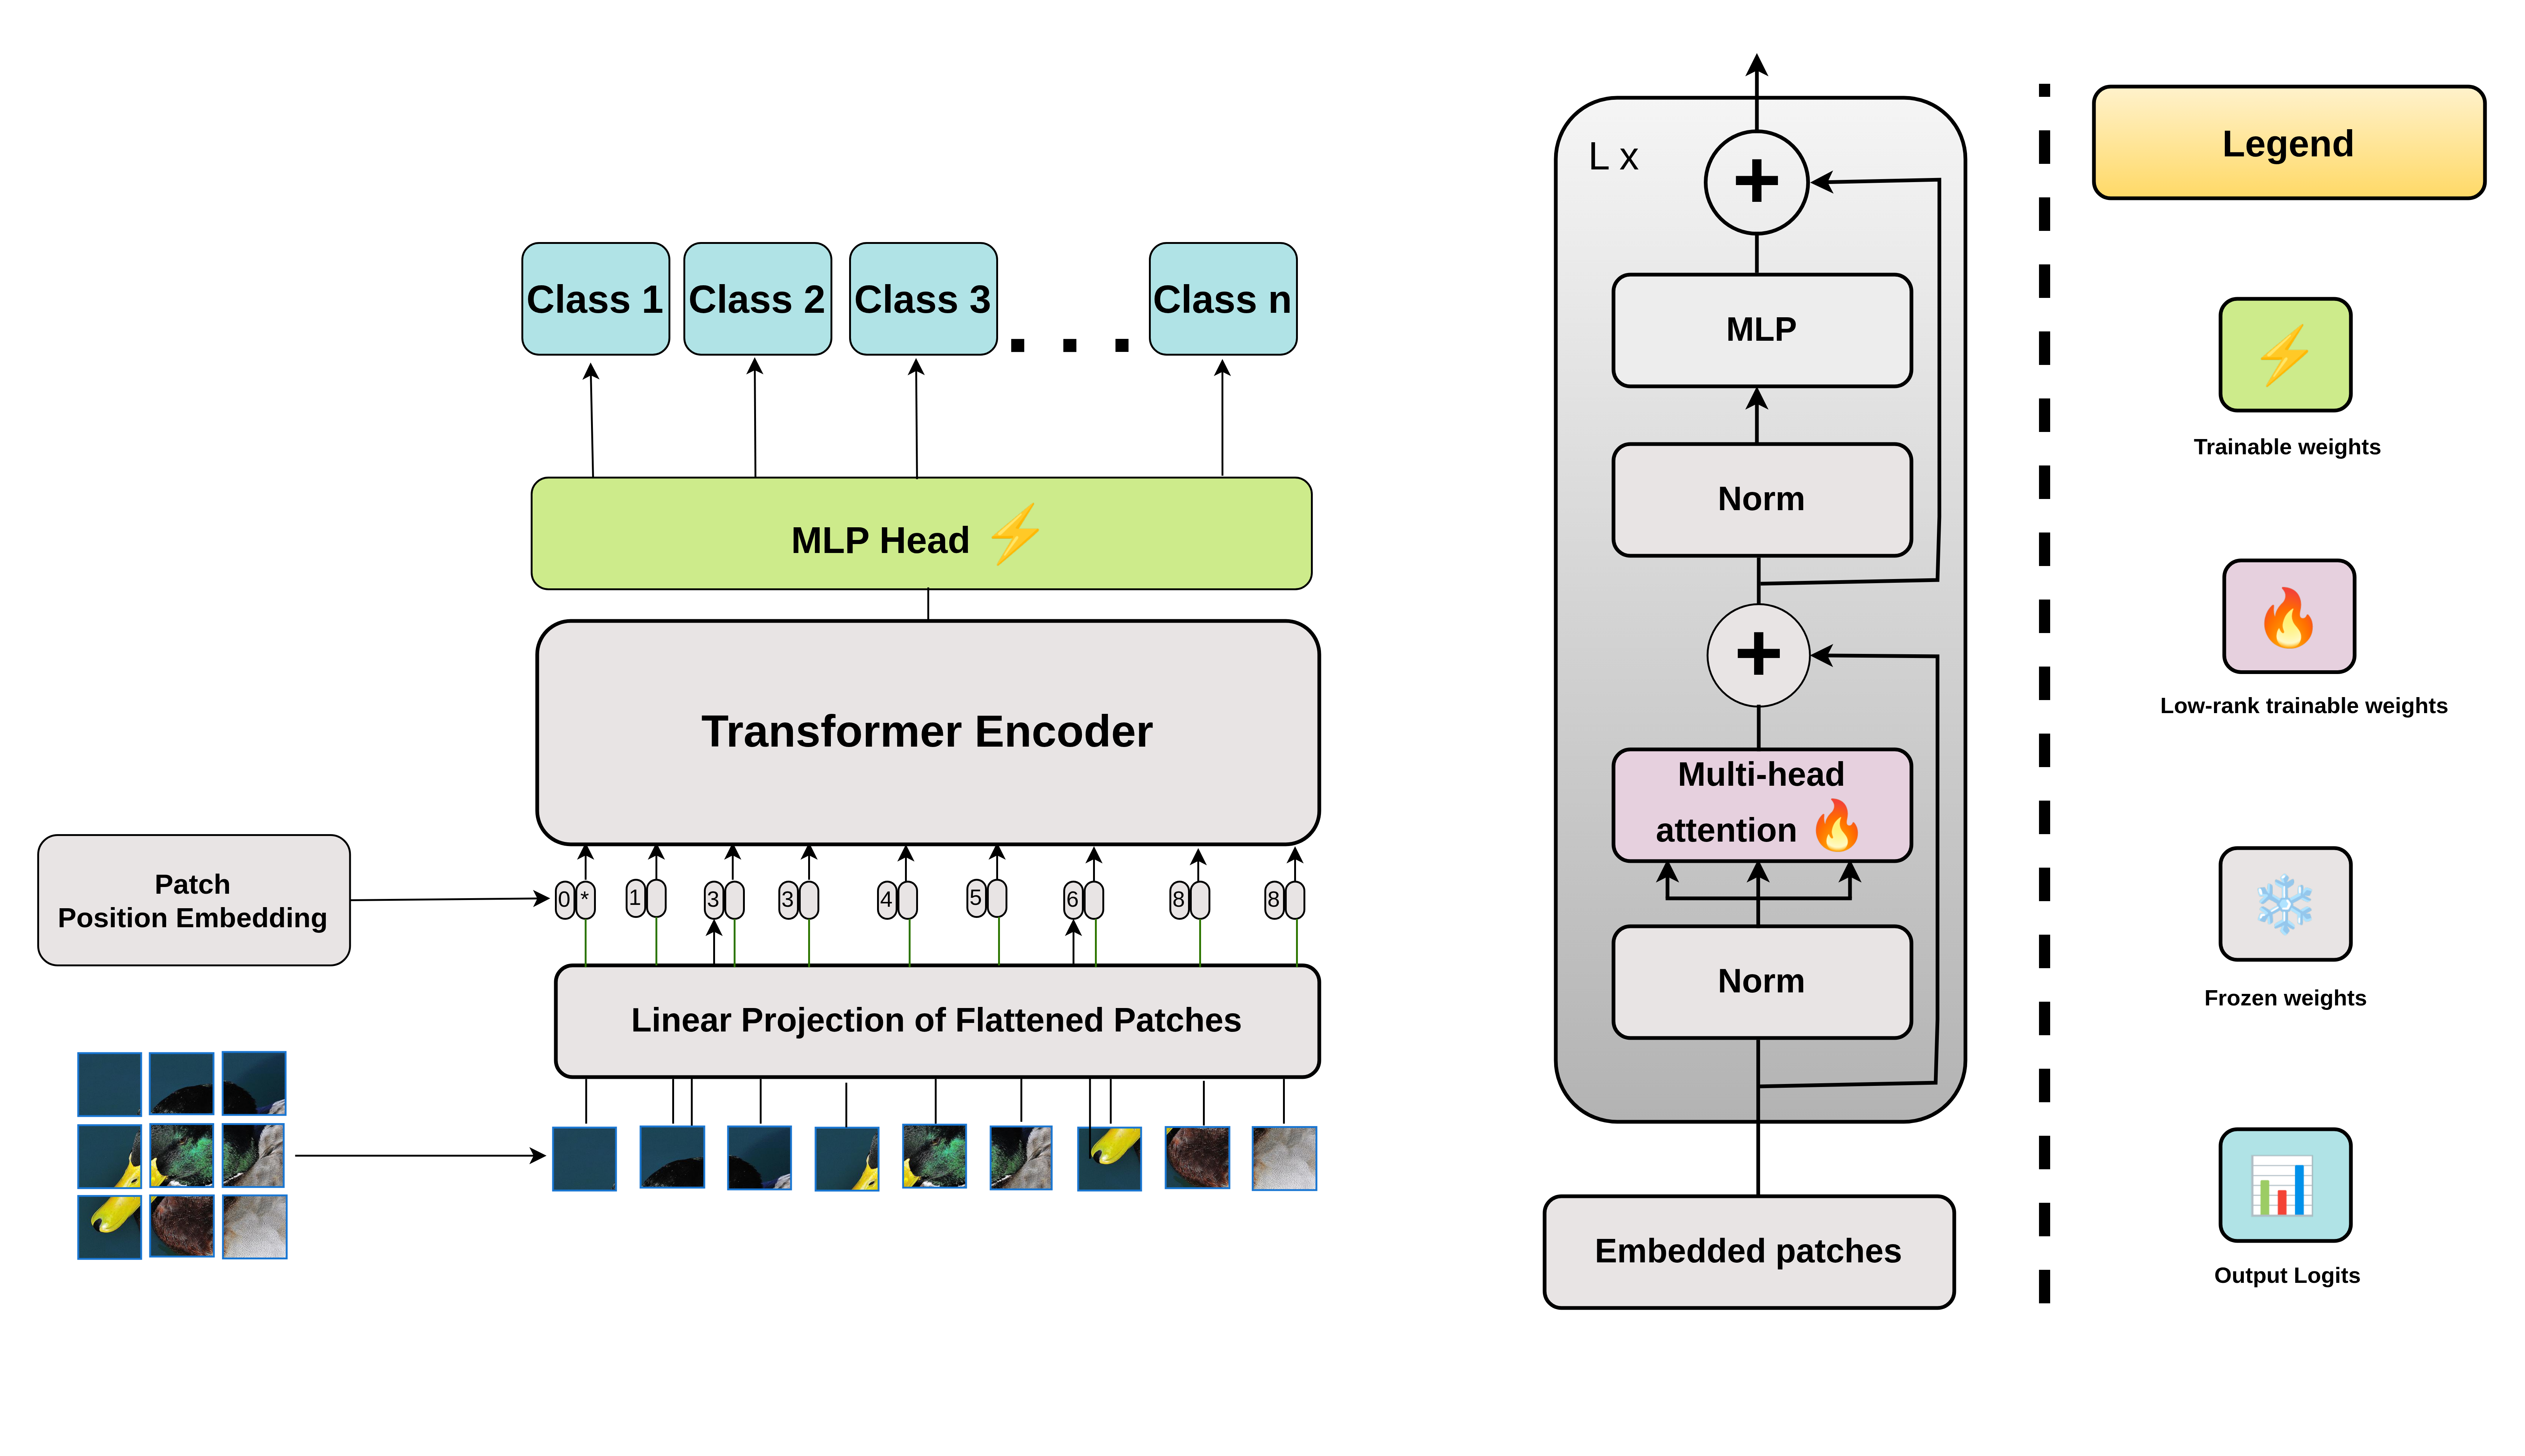
\includegraphics[width=0.75\textwidth]{images/Lora_Placement.png}
    \caption{LoRA placement in BID-LoRA at Attention Modules}
    \label{fig:BIDlora_pipeline}
\end{figure}

However, standard LoRA in CLU settings suffers from knowledge leakage gradual degradation of retained knowledge across successive steps (see Section~\ref{8.2}). \textcolor{red}{This is a direct consequence of shared parameterization: a single adapter's low-rank subspace $(B, A)$ must simultaneously satisfy retention, acquisition, and forgetting objectives within one cycle, whose gradients can point in conflicting directions within that same subspace, forcing each update to be a compromise between competing goals. Dedicating a disjoint low-rank subspace to each objective removes this conflict by construction: within a cycle, no objective's gradient can act on another's parameters, since they occupy physically separate matrices rather than a shared one. Each cycle's three adapters are freshly initialized and merged into the frozen base weights $W$ at the end of that cycle (Algorithm~\ref{alg:bidlora}); $W$, not the adapters, is therefore the only state carried across cycles, so a class's role transitioning from new to retained to forgotten over time is mediated by $W$'s accumulated updates, not by any adapter being reused across roles.}

\medskip
\noindent
\textit{Pathway Separation:}
To address cumulative knowledge drift, i.e., knowledge leakage, we dedicate distinct adapters to each objective: $W_f = B_{f}A_{f}$ for forgetting, $W_{\text{\textit{ret}}} = B_{\text{\textit{ret}}}A_{\text{\textit{ret}}}$ for retention, and $W_{\text{\textit{new}}} = B_{\text{\textit{new}}}A_{\text{\textit{new}}}$ for learning new classes. Critically, $W_f$ learns weights that \textit{nullify} forget-class knowledge, $W_{\text{\textit{new}}}$ acquires new knowledge, while $W_{\text{\textit{ret}}}$ preserves retained knowledge to counteract the knowledge leakage caused by both forget and new adapters. After sufficient training, adapters merge into the base weights $W$ as shown in Fig~\ref{fig:path_way_sepration}

\begin{equation}
h = Wx + \mathcal{S}\left(B_{\text{\textit{ret}}}A_{\text{\textit{ret}}} + B_{\text{\textit{new}}}A_{\text{\textit{new}}} + B_{\text{\textit{f}}}A_{\text{\textit{f}}}\right)x
\label{eq:merge}
\end{equation}
where $W \in \mathbb{R}^{d \times k}$ is frozen, and adapter consists of matrices $B_f,B_\text{\textit{ret}},B_\text{\textit{new}} \in \mathbb{R}^{d \times r}$ and $A_f,A_\text{\textit{ret}},A_\text{\textit{new}} \in \mathbb{R}^{r \times k}$ that serve their designated function. This separation provides two benefits: (1) drift in one adapter does not corrupt others, and (2) \textcolor{red}{each adapter's \textit{parameters} are updated only by its designated objective, without parameter interference from the other two pathways (gradients are still computed against the shared activation $h$, but only the designated adapter's weights are modified)}. Adapters merge at inference, preserving efficiency. We empirically validate pathway specialization in Section~\ref{7.4}.

\subsection{Loss Function}
\label{4.3}

In this section, we present the loss functions which are designed to balance forgetting, retention, and new knowledge acquisition in our continual adaptation framework.

\medskip
\noindent
\textit{Selective Forget Loss:}
Existing unlearning methods suffer from strong unlearning signals that degrade retention knowledge, resulting in improper forgetting. To address this, we propose \textit{Escape Unlearning}, a passive approach that pushes forget-class embeddings to an ``escape'' point maximally distant from all retain-class centroids, creating irreversible information loss. First, we compute the centroid of each class as:

\begin{figure}[!htbp]
    \centering
    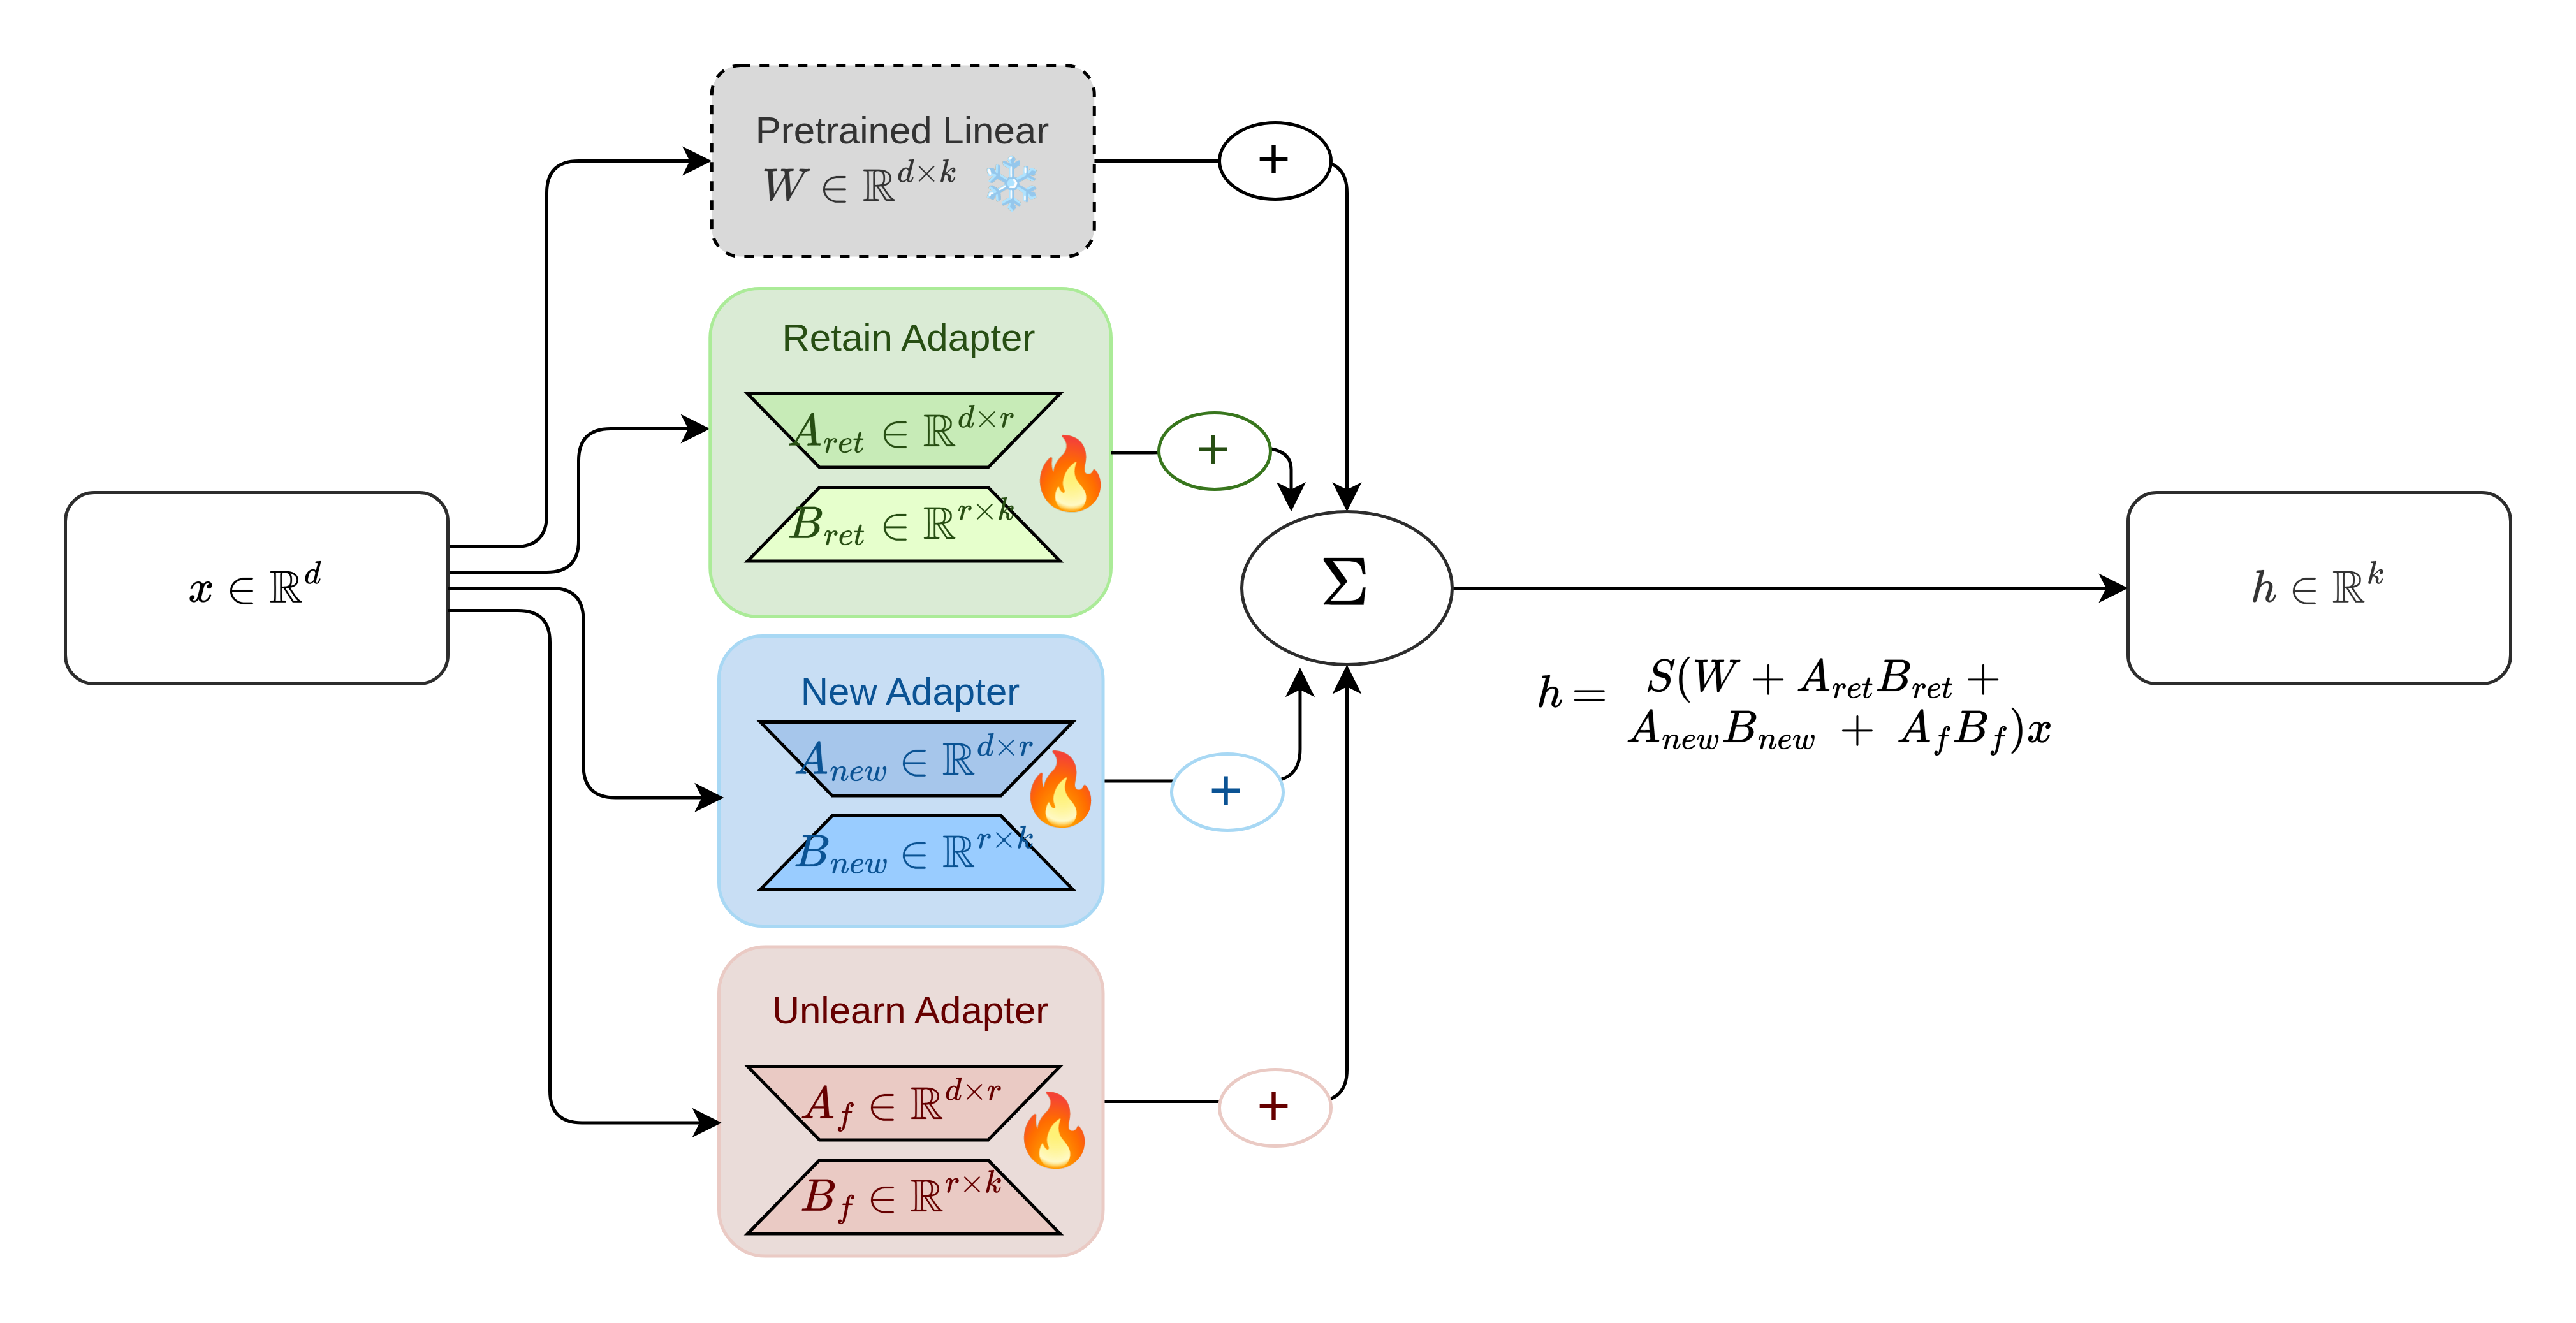
\includegraphics[width=0.75\linewidth]{images/pathwayas2.png}
    % \caption{Pathway separation for BID-LoRA, where \emoji{fire} indicates trainable and \emoji{snowflake} indicates frozen.}
    \caption{Pathway separation for BID-LoRA.}
    \label{fig:path_way_sepration}
\end{figure}

\begin{equation}
c_k = \frac{1}{|D_k|}\sum_{x \in D_k} \text{emb}(x)
\end{equation}

This yields retain centroids $\{c_{r_1}, c_{r_2}, \dots, c_{r_K}\}$ and forget centroids $\{c_{f_1}, c_{f_2}, \dots, c_{f_M}\}$. We obtain the escape direction by solving the minimax problem:
\begin{equation}
\mathbf{d}^* = \arg\min_{\|\mathbf{d}\|=1} \max_{i} \left( \mathbf{d}^\top c_{r_i} \right)
\end{equation}

where $\mathbf{d}^* \in \mathbb{R}^{\text{\textit{dim}}}$ is the escape direction vector in the $\textit{dim}$-dimensional embedding space, $\mathbf{d}^\top$ denotes the transpose, and $\mathbf{d}^\top c_{r_i}$ computes the dot product measuring the projection of retain centroid $c_{r_i}$ along direction $\mathbf{d}$. The constraint $\|\mathbf{d}\|=1$ ensures unit norm. The inner $\max_i$ identifies the retain centroid most aligned with $\mathbf{d}$, while the outer $\min$ searches over all unit directions to find $\mathbf{d}^*$ that minimizes this maximum alignment. Starting from a randomly initialized direction, the optimization iteratively converges to $\mathbf{d}^*$, yielding the direction maximally distant from all retain centroids.

\textcolor{red}{The forget adapter does not assign forgotten samples to another class. It pushes their embeddings toward a single escape point, computed via the minimax objective above to be equally far from every retain class centroid, rather than close to any one of them. Since the target is a point in embedding space and not a class label, the mechanism has no notion of a preferred wrong class to route samples toward. This distinguishes escape unlearning from systematic relabeling, where a model would be trained to consistently output one specific incorrect label (see Section~\ref{7.7} for the empirical Sink measurement that verifies this).}

However, placing the escape point on the unit sphere leads to unstable forgetting (see Section~\ref{7.6}). Therefore, we scale the escape point away from the sphere:

\begin{equation}
\mathbf{t}_{\text{escape}} = \lambda_{\text{esc}} \cdot \mathbf{d}^*
\end{equation}

This provides a target location away from retain embeddings in both direction and distance. The forget loss is then:
\begin{equation}
\mathcal{L}_{\text{\textit{f}}} = \text{MSE}\left( \text{emb}(\mathbf{X}^f), \mathbf{t}_{\text{escape}} \right)
\end{equation}

Where \text{MSE} indicates mean squared loss while this $\mathcal{L}_{\text{\textit{f}}}$ pushes all forget sample embeddings toward the escape point, creating a many-to-one mapping that destroys class-discriminative information.

\medskip
\noindent
\textit{Retention Loss}
The retention loss preserves knowledge of retain classes and prevents model drift toward the escape point through two complementary terms:
\begin{equation}
\mathcal{L}_{\text{\textit{ret}}} = \lambda_{\text{ce}} \cdot \text{CE}(\mathbf{z}_r, y_r) + \lambda_{\text{emb}} \cdot \text{MSE}(\mathbf{e}_r, \mathbf{e}_t)
\end{equation}

where $\mathbf{z}_r$ are student logits for retain samples, $y_r$ are ground truth labels, and $\mathbf{e}_r$, $\mathbf{e}_t$ are student and teacher embeddings respectively. The embedding anchor term $\text{MSE}(\mathbf{e}_r, \mathbf{e}_t)$ prevents representation drift by keeping student embeddings close to the teacher (i.e., away from escape point \textcolor{red}{$\mathbf{t}_{\text{escape}}$}), where the teacher is a frozen copy of the model at initialization.

\medskip
\noindent
\textit{New Knowledge Loss}
The model must simultaneously learn new classes using standard cross-entropy:
\begin{equation}
\mathcal{L}_{\text{\textit{new}}} = \text{CE}(\mathbf{z}_n, y_n)
\end{equation}

where \text{CE} indicates cross entropy loss $\mathbf{z}_n$ are logits and $y_n$ are labels for new class samples. 

\textcolor{red}{Although the three adapter outputs sum into the shared activation $h$ (Eq.~\ref{eq:merge}) during the forward pass, we isolate optimization at the parameter level: non-target adapters are frozen during each loss's backward pass, so gradients are never applied to their weights even though the forward computation is shared. Consequently each loss updates only its designated adapter and corresponding classifier-head nodes, without altering the other two pathways.} During gradient updates, non-target adapters are frozen and non-target head gradients are masked to zero. Specifically, $\mathcal{L}_{\text{\textit{f}}}$, $\mathcal{L}_{\text{\textit{ret}}}$, and $\mathcal{L}_{\text{\textit{new}}}$ update only their respective adapters $(B, A)$ and corresponding classifier head nodes. This ensures forgetting cannot corrupt retained knowledge and each adapter specializes to its function, as per assumption~2 (Section~\ref{3.2}), if only learning or unlearning is required, the corresponding loss terms are masked accordingly.

\textcolor{red}{
\noindent\textbf{Classifier-head handling.}
The classification head is a single linear layer with one output node per class, incrementally extended whenever new classes are introduced. At each step $t$, its nodes are partitioned into retain-, forget-, and new-class subsets; the masking scheme described above (non-target gradients masked to zero) applies identically to the head, so a given loss updates only its corresponding subset of head nodes. At the following step, nodes that were new-class at step $t$ are reclassified as retain-class nodes, while forgotten nodes from step $t$ remain excluded going forward. After merging, we remove the head's forget-class output nodes entirely, consistent with the adapter-deletion rationale of Assumption~4 (Section~\ref{3.2}): since escape unlearning collapses forget-class embeddings to a single point, their corresponding head weights carry no discriminative signal, and retaining them would needlessly expose which classes were removed.
}

\textcolor{red}{
\noindent\textbf{Why adapter deletion is necessary.}
After merging, the adapted model satisfies $\mathcal{M}' = \mathcal{M}_\text{orig} \oplus \mathcal{S}(B_\text{ret}A_\text{ret} + B_\text{new}A_\text{new} + B_f A_f)$. If all adapter matrices are retained, an adversary can exactly reconstruct the pre-adaptation model as shown below
\begin{equation}
\mathcal{M}_\text{orig} = \mathcal{M}' \ominus \mathcal{S}\!\left(B_\text{ret}A_\text{ret} + B_\text{new}A_\text{new} + B_f A_f\right),
\label{eq:recovery}
\end{equation}
fully recovering all unlearned knowledge. Permanent deletion of adapter matrices and $\mathcal{M}_\text{orig}$ post-merge eliminates this inversion, making recovery computationally intractable (Assumption~4, Section~\ref{3.2}).
}

\label{4.4}
Algorithm~\ref{alg:bidlora} summarizes the complete BID-LoRA training procedure. Each iteration performs gradient-isolated updates for retain, forget, and new pathways sequentially, ensuring no cross-pathway interference. After training, adapters merge into base weights for efficient inference. \textcolor{red}{Delete all adapters post-merge (Assumption~4).}
\begin{algorithm}[!htbp]
\caption{BID-LoRA Training}
\label{alg:bidlora} 
\begin{algorithmic}[1]
\Require Pre-trained model $\mathcal{M}$, retain data $D^\text{\textit{full}}_r$, forget data $D_f$, new data $D_\text{\textit{new}}$, replay buffer $D_r$ 
and $\mathcal{S}$ be the LoRA scaling factor
\Ensure Updated model with merged adapters

\State Initialize adapters $(B_{\text{\textit{ret}}}, A_{\text{\textit{ret}}})$, $(B_{\text{\textit{new}}}, A_{\text{\textit{new}}})$, $(B_{\text{\textit{f}}}, A_{\text{\textit{f}}})$
\State Freeze backbone weights $W$
\State $\mathcal{M_\text{\textit{t}}} \gets \text{copy}(\mathcal{M})$ \Comment{Frozen teacher for embedding anchor}

\State \textbf{// Compute escape point}
\For{each class $k$ in $D_r$}
    \State $c_k \gets \frac{1}{|D_k|}\sum_{x \in D_k} \text{emb}(x)$ \Comment{Retain centroids}
\EndFor
\State $\mathbf{d}^* \gets \arg\min_{\|\mathbf{d}\|=1} \max_{i} (\mathbf{d}^\top c_{r_i})$ \Comment{Escape direction}
\State $\mathbf{t}_{\text{escape}} \gets \lambda_{\text{esc}} \cdot \mathbf{d}^*$ \Comment{Escape point}

\For{epoch $= 1$ to $E$}
    % \For{each mini-batch $(X_\text{\textit{ret}}, X_\text{\textit{f}}, X_\text{\textit{new}})$}
    \For{each mini-batch $(X_\textit{ret}, y_\textit{ret}), (X_f, y_f), (X_\textit{new}, y_\textit{new})$ from $(D_r, D_f, D_\textit{new})$}
        \State \textbf{// Retention update}
        \State Freeze $(B_{\text{f}}, A_{\text{f}})$, $(B_{\text{new}}, A_{\text{new}})$
        \State $\mathbf{z}_\text{\textit{ret}} \gets \mathcal{M}(X_\text{\textit{ret}})$ \Comment{Student logits}
        \State $\mathbf{e}_\text{\textit{ret}} \gets \text{emb}(X_\text{\textit{ret}})$ \Comment{Student embeddings}
        \State $\mathbf{e}_\textit{ret,t} \gets \mathcal{M}_t.\text{emb}(X_\text{\textit{ret}})$ \Comment{Teacher embeddings}
        \State $\mathcal{L}_{\text{ret}} \gets \lambda_{\text{ce}} \cdot \text{CE}(\mathbf{z}_\textit{ret}, y_\textit{ret}) + \lambda_{\text{emb}} \cdot \text{MSE}(\mathbf{e}_\textit{ret}, \mathbf{e}_\textit{t,ret})$
        \State Update $(B_{\text{ret}}, A_{\text{ret}})$ and retain-class head
        
        \State \textbf{// Forget update}
        \State Freeze $(B_{\text{\textit{ret}}}, A_{\text{\textit{ret}}})$, $(B_{\text{\textit{new}}}, A_{\text{\textit{new}}})$
        \State $\mathcal{L}_{\text{forget}} \gets \text{MSE}(\text{emb}(X_\text{\textit{f}}), \mathbf{t}_{\text{escape}})$
        \State Update $(B_{\text{\textit{f}}}, A_{\text{\textit{f}}})$ and forget-class head
        
        \State \textbf{// New knowledge update}
        \State Freeze $(B_{\text{\textit{ret}}}, A_{\text{\textit{ret}}})$, $(B_{\text{\textit{f}}}, A_{\text{\textit{f}}})$
        \State $\mathcal{L}_{\text{\textit{new}}} \gets \text{CE}(\mathcal{M}(X_\text{\textit{new}}), y_n)$
        \State Update $(B_{\text{\textit{new}}}, A_{\text{\textit{new}}})$ and new-class head
    \EndFor
\EndFor

\State \textbf{// Merge adapters}
\State \textcolor{red}{$W \gets W + \mathcal{S}(B_{\text{\textit{ret}}}A_{\text{\textit{ret}}} + B_{\text{\textit{new}}}A_{\text{\textit{new}}} + B_{\text{\textit{f}}}A_{\text{\textit{f}}})$}
\State \textcolor{red}{\textbf{Delete} $(B_f, A_f)$, $(B_\text{\textit{ret}}, A_\text{\textit{ret}})$, $(B_\text{\textit{new}}, A_\text{\textit{new}})$, pre-adaptation checkpoint $\mathcal{M}_\text{orig}$, and forget-class head nodes}

\State \Return $\mathcal{M}$
\end{algorithmic}
\end{algorithm}

\begin{table}[!htbp]
\centering
\renewcommand{\arraystretch}{1.30}
\caption{Performance comparison across all continual learning-unlearning tasks on CIFAR-100. \textcolor{red}{KL divergence and MIA are reported in the ablation study (Section~\ref{7.0}). BID-LoRA results are mean$_{\pm\text{std}}$ over 3 seeds.}}
\label{tab:classification}
\begin{adjustbox}{max width=\textwidth}
\setlength{\tabcolsep}{3pt}
\begin{tabular}{l|c|cccc|cccc}
\toprule
\multirow{2}{*}{\textbf{Method}} & \multirow{2}{*}{\textbf{Tunable} $\downarrow$}
& \multicolumn{4}{c|}{\textbf{Task-1}} & \multicolumn{4}{c}{\textbf{Task-2}} \\
\cmidrule(lr){3-6} \cmidrule(lr){7-10}
& & $Acc_f \downarrow$ & $Acc_r \uparrow$ & $Acc_n \uparrow$ & $Acc_o \uparrow$
& $Acc_f \downarrow$ & $Acc_r \uparrow$ & $Acc_n \uparrow$ & $Acc_o \uparrow$ \\
\midrule
Oracle        & 100\% & -- & -- & -- & 78.89 & -- & -- & -- & 75.60 \\
\midrule
LSF           & 100\% & 0.00 & 70.21 & 80.23 & 73.55 & 0.00 & 70.31 & 78.27 & 72.96 \\
CLPU-DER++    & 100\% & 0.27 & 70.30 & 70.27 & 70.29 & 0.00 & 68.32 & 73.47 & 70.04 \\
UniCLUN       & 100\% & 2.37 & 72.39 & 75.32 & 73.37 & 0.20 & 67.27 & 74.63 & 69.72 \\
UG-CLU        & 100\% & 1.31 & 76.73 & 73.27 & 75.58 & 0.37 & 70.32 & 71.47 & 70.70 \\
UnCLe         & 100\% & 1.47 & 78.43 & 75.23 & 76.83 & 0.50 & 70.00 & 76.27 & 72.09 \\
\midrule
\rowcolor{pink!15}
\textbf{BID-LoRA} & 5.08\% & $\kern6pt0.93_{\scriptscriptstyle \pm 0.08}\kern-6pt$ & $\kern6pt75.71_{\scriptscriptstyle \pm 0.31}\kern-6pt$ & $\kern6pt76.93_{\scriptscriptstyle \pm 0.28}\kern-6pt$ & $\kern6pt76.03_{\scriptscriptstyle \pm 0.24}\kern-6pt$ & $\kern6pt0.27_{\scriptscriptstyle \pm 0.04}\kern-6pt$ & $\kern6pt70.83_{\scriptscriptstyle \pm 0.27}\kern-6pt$ & $\kern6pt79.87_{\scriptscriptstyle \pm 0.35}\kern-6pt$ & $\kern6pt73.84_{\scriptscriptstyle \pm 0.29}\kern-6pt$ \\
\midrule
\addlinespace[0.2cm]
\midrule
\multirow{2}{*}{\textbf{Method}} & \multirow{2}{*}{\textbf{Tunable} $\downarrow$}
& \multicolumn{4}{c|}{\textbf{Task-3}} & \multicolumn{4}{c}{\textbf{Task-4}} \\
\cmidrule(lr){3-6} \cmidrule(lr){7-10}
& & $Acc_f \downarrow$ & $Acc_r \uparrow$ & $Acc_n \uparrow$ & $Acc_o \uparrow$
& $Acc_f \downarrow$ & $Acc_r \uparrow$ & $Acc_n \uparrow$ & $Acc_o \uparrow$ \\
\midrule
Oracle        & 100\% & -- & -- & -- & 77.64 & -- & -- & -- & 78.04 \\
\midrule
LSF           & 100\% & 1.00 & 72.00 & 77.25 & 73.75 & 0.00 & 75.00 & 73.35 & 74.45 \\
CLPU-DER++    & 100\% & 0.48 & 71.33 & 80.25 & 74.31 & 0.25 & 79.28 & 72.25 & 76.94 \\
UniCLUN       & 100\% & 0.36 & 68.48 & 79.00 & 71.99 & 0.36 & 73.25 & 70.89 & 72.46 \\
UG-CLU        & 100\% & 0.00 & 74.58 & 78.25 & 75.81 & 0.00 & 70.25 & 74.89 & 71.80 \\
UnCLe         & 100\% & 0.00 & 71.00 & 81.25 & 74.42 & 0.89 & 74.36 & 71.58 & 73.43 \\
\midrule
\rowcolor{pink!15}
\textbf{BID-LoRA} & 5.08\% & $\kern6pt0.13_{\scriptscriptstyle \pm 0.02}\kern-6pt$ & $\kern6pt72.33_{\scriptscriptstyle \pm 0.19}\kern-6pt$ & $\kern6pt79.73_{\scriptscriptstyle \pm 0.31}\kern-6pt$ & $\kern6pt74.80_{\scriptscriptstyle \pm 0.22}\kern-6pt$ & $\kern6pt0.27_{\scriptscriptstyle \pm 0.04}\kern-6pt$ & $\kern6pt76.00_{\scriptscriptstyle \pm 0.23}\kern-6pt$ & $\kern6pt78.13_{\scriptscriptstyle \pm 0.27}\kern-6pt$ & $\kern6pt76.71_{\scriptscriptstyle \pm 0.20}\kern-6pt$ \\
\midrule
\addlinespace[0.2cm]
\midrule
\multirow{2}{*}{\textbf{Method}} & \multirow{2}{*}{\textbf{Tunable} $\downarrow$}
& \multicolumn{4}{c|}{\textbf{Task-5}} & \multicolumn{4}{c}{\textbf{Task-6}} \\
\cmidrule(lr){3-6} \cmidrule(lr){7-10}
& & $Acc_f \downarrow$ & $Acc_r \uparrow$ & $Acc_n \uparrow$ & $Acc_o \uparrow$
& $Acc_f \downarrow$ & $Acc_r \uparrow$ & $Acc_n \uparrow$ & $Acc_o \uparrow$ \\
\midrule
Oracle        & 100\% & -- & -- & -- & 78.44 & -- & -- & -- & 79.16 \\
\midrule
LSF           & 100\% & 0.00 & 68.98 & 78.91 & 73.75 & 0.00 & 65.00 & 75.37 & 68.46 \\
CLPU-DER++    & 100\% & 0.00 & 69.00 & 75.89 & 74.31 & 0.87 & 67.81 & 79.87 & 71.83 \\
UniCLUN       & 100\% & 0.22 & 73.25 & 74.25 & 71.99 & 0.00 & 68.50 & 83.00 & 73.33 \\
UG-CLU        & 100\% & 0.00 & 71.35 & 76.36 & 75.81 & 0.00 & 63.51 & 81.29 & 69.44 \\
UnCLe         & 100\% & 0.87 & 70.98 & 77.82 & 74.42 & 0.00 & 67.00 & 80.00 & 71.33 \\
\midrule
\rowcolor{pink!15}
\textbf{BID-LoRA} & 5.08\% & $\kern6pt0.67_{\scriptscriptstyle \pm 0.07}\kern-6pt$ & $\kern6pt72.33_{\scriptscriptstyle \pm 0.26}\kern-6pt$ & $\kern6pt80.80_{\scriptscriptstyle \pm 0.33}\kern-6pt$ & $\kern6pt75.16_{\scriptscriptstyle \pm 0.24}\kern-6pt$ & $\kern6pt0.00_{\scriptscriptstyle \pm 0.00}\kern-6pt$ & $\kern6pt68.67_{\scriptscriptstyle \pm 0.21}\kern-6pt$ & $\kern6pt83.20_{\scriptscriptstyle \pm 0.29}\kern-6pt$ & $\kern6pt73.51_{\scriptscriptstyle \pm 0.19}\kern-6pt$ \\
\bottomrule
\end{tabular}
\end{adjustbox}
\end{table}

% !!! PLACEHOLDER NUMBERS in tab:face_recognition -- VGGFace2 (200 identities), 12-task
% sliding-window protocol. Every value below is DUMMY, generated to follow the same
% trend as the CASIA-Face100 results (Table 1). Replace with real measurements before
% submission.
\begin{table}[!htbp]
\centering
\renewcommand{\arraystretch}{1.30}
\caption{\textcolor{red}{Performance comparison across all 12 continual learning-unlearning tasks on Face Recognition on VGGFace2 (200 identities). KL divergence and MIA are reported in the ablation study (Section~\ref{7.0}). BID-LoRA results are mean$_{\pm\text{std}}$ over 3 seeds. Values shown are placeholder/dummy, pending real experiments.}}
\label{tab:face_recognition}
\begin{adjustbox}{max width=\textwidth}
\setlength{\tabcolsep}{3pt}
\begin{tabular}{l|c|cccc|cccc}
\toprule
\multirow{2}{*}{\textbf{Method}} & \multirow{2}{*}{\textbf{Tunable} $\downarrow$}
& \multicolumn{4}{c|}{\textbf{Task-1}} & \multicolumn{4}{c}{\textbf{Task-2}} \\
\cmidrule(lr){3-6} \cmidrule(lr){7-10}
& & $Acc_f \downarrow$ & $Acc_r \uparrow$ & $Acc_n \uparrow$ & $Acc_o \uparrow$
& $Acc_f \downarrow$ & $Acc_r \uparrow$ & $Acc_n \uparrow$ & $Acc_o \uparrow$ \\
\midrule
Oracle        & 100\% & -- & -- & -- & 95.83 & -- & -- & -- & 94.32 \\
\midrule
LSF           & 100\% & 0.03 & 88.38 & 90.12 & 88.96 & 0.81 & 90.49 & 90.70 & 90.56 \\
CLPU-DER++    & 100\% & 0.74 & 90.38 & 93.46 & 91.41 & 0.16 & 91.79 & 90.68 & 91.42 \\
UniCLUN       & 100\% & 0.09 & 89.11 & 89.15 & 89.12 & 0.09 & 87.48 & 93.24 & 89.40 \\
UG-CLU        & 100\% & 0.22 & 89.53 & 89.13 & 89.40 & 0.60 & 91.04 & 92.65 & 91.58 \\
UnCLe         & 100\% & 0.20 & 90.25 & 91.72 & 90.74 & 0.54 & 91.87 & 90.89 & 91.54 \\
\midrule
\rowcolor{pink!15}
\textbf{BID-LoRA} & 5.00\% & $\kern6pt0.20_{\scriptscriptstyle \pm 0.05}\kern-6pt$ & $\kern6pt91.98_{\scriptscriptstyle \pm 0.22}\kern-6pt$ & $\kern6pt94.12_{\scriptscriptstyle \pm 0.19}\kern-6pt$ & $\kern6pt92.69_{\scriptscriptstyle \pm 0.20}\kern-6pt$ & $\kern6pt0.50_{\scriptscriptstyle \pm 0.05}\kern-6pt$ & $\kern6pt92.46_{\scriptscriptstyle \pm 0.22}\kern-6pt$ & $\kern6pt93.74_{\scriptscriptstyle \pm 0.19}\kern-6pt$ & $\kern6pt92.89_{\scriptscriptstyle \pm 0.20}\kern-6pt$ \\
\midrule
\addlinespace[0.2cm]
\midrule
\multirow{2}{*}{\textbf{Method}} & \multirow{2}{*}{\textbf{Tunable} $\downarrow$}
& \multicolumn{4}{c|}{\textbf{Task-3}} & \multicolumn{4}{c}{\textbf{Task-4}} \\
\cmidrule(lr){3-6} \cmidrule(lr){7-10}
& & $Acc_f \downarrow$ & $Acc_r \uparrow$ & $Acc_n \uparrow$ & $Acc_o \uparrow$
& $Acc_f \downarrow$ & $Acc_r \uparrow$ & $Acc_n \uparrow$ & $Acc_o \uparrow$ \\
\midrule
Oracle        & 100\% & -- & -- & -- & 96.37 & -- & -- & -- & 96.05 \\
\midrule
LSF           & 100\% & 0.58 & 90.52 & 89.23 & 90.09 & 0.16 & 88.90 & 93.95 & 90.58 \\
CLPU-DER++    & 100\% & 0.23 & 88.45 & 89.40 & 88.77 & 0.64 & 89.78 & 92.42 & 90.66 \\
UniCLUN       & 100\% & 0.23 & 87.51 & 90.39 & 88.47 & 0.84 & 90.88 & 90.15 & 90.64 \\
UG-CLU        & 100\% & 0.64 & 88.82 & 90.85 & 89.50 & 0.03 & 88.58 & 90.34 & 89.17 \\
UnCLe         & 100\% & 0.21 & 88.33 & 93.68 & 90.11 & 0.21 & 91.71 & 93.38 & 92.27 \\
\midrule
\rowcolor{pink!15}
\textbf{BID-LoRA} & 5.00\% & $\kern6pt0.58_{\scriptscriptstyle \pm 0.05}\kern-6pt$ & $\kern6pt92.02_{\scriptscriptstyle \pm 0.22}\kern-6pt$ & $\kern6pt92.84_{\scriptscriptstyle \pm 0.19}\kern-6pt$ & $\kern6pt92.29_{\scriptscriptstyle \pm 0.20}\kern-6pt$ & $\kern6pt0.28_{\scriptscriptstyle \pm 0.05}\kern-6pt$ & $\kern6pt92.11_{\scriptscriptstyle \pm 0.22}\kern-6pt$ & $\kern6pt93.29_{\scriptscriptstyle \pm 0.19}\kern-6pt$ & $\kern6pt92.50_{\scriptscriptstyle \pm 0.20}\kern-6pt$ \\
\midrule
\addlinespace[0.2cm]
\midrule
\multirow{2}{*}{\textbf{Method}} & \multirow{2}{*}{\textbf{Tunable} $\downarrow$}
& \multicolumn{4}{c|}{\textbf{Task-5}} & \multicolumn{4}{c}{\textbf{Task-6}} \\
\cmidrule(lr){3-6} \cmidrule(lr){7-10}
& & $Acc_f \downarrow$ & $Acc_r \uparrow$ & $Acc_n \uparrow$ & $Acc_o \uparrow$
& $Acc_f \downarrow$ & $Acc_r \uparrow$ & $Acc_n \uparrow$ & $Acc_o \uparrow$ \\
\midrule
Oracle        & 100\% & -- & -- & -- & 96.49 & -- & -- & -- & 95.22 \\
\midrule
LSF           & 100\% & 0.46 & 88.32 & 90.23 & 88.96 & 1.00 & 89.65 & 93.86 & 91.05 \\
CLPU-DER++    & 100\% & 0.56 & 88.31 & 91.92 & 89.51 & 0.86 & 87.06 & 92.60 & 88.91 \\
UniCLUN       & 100\% & 0.90 & 89.00 & 90.10 & 89.37 & 0.68 & 89.68 & 90.33 & 89.90 \\
UG-CLU        & 100\% & 1.00 & 89.55 & 89.45 & 89.52 & 0.64 & 87.56 & 91.17 & 88.76 \\
UnCLe         & 100\% & 0.05 & 87.55 & 92.14 & 89.08 & 0.45 & 91.77 & 93.38 & 92.31 \\
\midrule
\rowcolor{pink!15}
\textbf{BID-LoRA} & 5.00\% & $\kern6pt0.71_{\scriptscriptstyle \pm 0.05}\kern-6pt$ & $\kern6pt91.64_{\scriptscriptstyle \pm 0.22}\kern-6pt$ & $\kern6pt92.63_{\scriptscriptstyle \pm 0.19}\kern-6pt$ & $\kern6pt91.97_{\scriptscriptstyle \pm 0.20}\kern-6pt$ & $\kern6pt0.24_{\scriptscriptstyle \pm 0.05}\kern-6pt$ & $\kern6pt91.80_{\scriptscriptstyle \pm 0.22}\kern-6pt$ & $\kern6pt92.86_{\scriptscriptstyle \pm 0.19}\kern-6pt$ & $\kern6pt92.15_{\scriptscriptstyle \pm 0.20}\kern-6pt$ \\
\midrule
\addlinespace[0.2cm]
\midrule
\multirow{2}{*}{\textbf{Method}} & \multirow{2}{*}{\textbf{Tunable} $\downarrow$}
& \multicolumn{4}{c|}{\textbf{Task-7}} & \multicolumn{4}{c}{\textbf{Task-8}} \\
\cmidrule(lr){3-6} \cmidrule(lr){7-10}
& & $Acc_f \downarrow$ & $Acc_r \uparrow$ & $Acc_n \uparrow$ & $Acc_o \uparrow$
& $Acc_f \downarrow$ & $Acc_r \uparrow$ & $Acc_n \uparrow$ & $Acc_o \uparrow$ \\
\midrule
Oracle        & 100\% & -- & -- & -- & 96.49 & -- & -- & -- & 96.57 \\
\midrule
LSF           & 100\% & 0.87 & 88.49 & 92.19 & 89.72 & 0.09 & 89.43 & 89.35 & 89.40 \\
CLPU-DER++    & 100\% & 0.61 & 87.76 & 92.81 & 89.44 & 0.76 & 90.83 & 89.64 & 90.43 \\
UniCLUN       & 100\% & 0.54 & 90.89 & 91.65 & 91.14 & 0.48 & 89.75 & 90.33 & 89.94 \\
UG-CLU        & 100\% & 0.00 & 88.62 & 89.10 & 88.78 & 0.87 & 89.12 & 90.06 & 89.43 \\
UnCLe         & 100\% & 0.93 & 91.39 & 93.16 & 91.98 & 0.54 & 90.65 & 90.01 & 90.44 \\
\midrule
\rowcolor{pink!15}
\textbf{BID-LoRA} & 5.00\% & $\kern6pt0.28_{\scriptscriptstyle \pm 0.05}\kern-6pt$ & $\kern6pt90.92_{\scriptscriptstyle \pm 0.22}\kern-6pt$ & $\kern6pt94.26_{\scriptscriptstyle \pm 0.19}\kern-6pt$ & $\kern6pt92.03_{\scriptscriptstyle \pm 0.20}\kern-6pt$ & $\kern6pt0.28_{\scriptscriptstyle \pm 0.05}\kern-6pt$ & $\kern6pt92.79_{\scriptscriptstyle \pm 0.22}\kern-6pt$ & $\kern6pt93.80_{\scriptscriptstyle \pm 0.19}\kern-6pt$ & $\kern6pt93.13_{\scriptscriptstyle \pm 0.20}\kern-6pt$ \\
\midrule
\addlinespace[0.2cm]
\midrule
\multirow{2}{*}{\textbf{Method}} & \multirow{2}{*}{\textbf{Tunable} $\downarrow$}
& \multicolumn{4}{c|}{\textbf{Task-9}} & \multicolumn{4}{c}{\textbf{Task-10}} \\
\cmidrule(lr){3-6} \cmidrule(lr){7-10}
& & $Acc_f \downarrow$ & $Acc_r \uparrow$ & $Acc_n \uparrow$ & $Acc_o \uparrow$
& $Acc_f \downarrow$ & $Acc_r \uparrow$ & $Acc_n \uparrow$ & $Acc_o \uparrow$ \\
\midrule
Oracle        & 100\% & -- & -- & -- & 95.35 & -- & -- & -- & 95.67 \\
\midrule
LSF           & 100\% & 0.52 & 87.61 & 90.12 & 88.45 & 0.47 & 90.92 & 93.04 & 91.63 \\
CLPU-DER++    & 100\% & 0.34 & 89.94 & 90.15 & 90.01 & 0.19 & 87.48 & 91.16 & 88.71 \\
UniCLUN       & 100\% & 0.22 & 87.35 & 92.16 & 88.95 & 0.42 & 89.34 & 92.65 & 90.44 \\
UG-CLU        & 100\% & 0.23 & 91.53 & 93.30 & 92.12 & 0.67 & 91.92 & 89.49 & 91.11 \\
UnCLe         & 100\% & 0.07 & 88.19 & 92.34 & 89.57 & 0.40 & 88.70 & 93.31 & 90.24 \\
\midrule
\rowcolor{pink!15}
\textbf{BID-LoRA} & 5.00\% & $\kern6pt0.19_{\scriptscriptstyle \pm 0.05}\kern-6pt$ & $\kern6pt91.06_{\scriptscriptstyle \pm 0.22}\kern-6pt$ & $\kern6pt94.37_{\scriptscriptstyle \pm 0.19}\kern-6pt$ & $\kern6pt92.16_{\scriptscriptstyle \pm 0.20}\kern-6pt$ & $\kern6pt0.22_{\scriptscriptstyle \pm 0.05}\kern-6pt$ & $\kern6pt91.18_{\scriptscriptstyle \pm 0.22}\kern-6pt$ & $\kern6pt93.40_{\scriptscriptstyle \pm 0.19}\kern-6pt$ & $\kern6pt91.92_{\scriptscriptstyle \pm 0.20}\kern-6pt$ \\
\midrule
\addlinespace[0.2cm]
\midrule
\multirow{2}{*}{\textbf{Method}} & \multirow{2}{*}{\textbf{Tunable} $\downarrow$}
& \multicolumn{4}{c|}{\textbf{Task-11}} & \multicolumn{4}{c}{\textbf{Task-12}} \\
\cmidrule(lr){3-6} \cmidrule(lr){7-10}
& & $Acc_f \downarrow$ & $Acc_r \uparrow$ & $Acc_n \uparrow$ & $Acc_o \uparrow$
& $Acc_f \downarrow$ & $Acc_r \uparrow$ & $Acc_n \uparrow$ & $Acc_o \uparrow$ \\
\midrule
Oracle        & 100\% & -- & -- & -- & 95.31 & -- & -- & -- & 96.66 \\
\midrule
LSF           & 100\% & 0.28 & 88.25 & 93.62 & 90.04 & 0.27 & 90.92 & 91.28 & 91.04 \\
CLPU-DER++    & 100\% & 0.44 & 91.31 & 91.75 & 91.46 & 0.42 & 91.79 & 93.98 & 92.52 \\
UniCLUN       & 100\% & 0.05 & 92.00 & 93.18 & 92.39 & 0.56 & 90.59 & 89.77 & 90.32 \\
UG-CLU        & 100\% & 0.97 & 91.63 & 93.24 & 92.17 & 0.30 & 91.84 & 91.90 & 91.86 \\
UnCLe         & 100\% & 0.17 & 89.43 & 90.07 & 89.64 & 0.54 & 90.74 & 89.29 & 90.26 \\
\midrule
\rowcolor{pink!15}
\textbf{BID-LoRA} & 5.00\% & $\kern6pt0.36_{\scriptscriptstyle \pm 0.05}\kern-6pt$ & $\kern6pt90.92_{\scriptscriptstyle \pm 0.22}\kern-6pt$ & $\kern6pt93.26_{\scriptscriptstyle \pm 0.19}\kern-6pt$ & $\kern6pt91.70_{\scriptscriptstyle \pm 0.20}\kern-6pt$ & $\kern6pt0.53_{\scriptscriptstyle \pm 0.05}\kern-6pt$ & $\kern6pt91.81_{\scriptscriptstyle \pm 0.22}\kern-6pt$ & $\kern6pt94.21_{\scriptscriptstyle \pm 0.19}\kern-6pt$ & $\kern6pt92.61_{\scriptscriptstyle \pm 0.20}\kern-6pt$ \\

\bottomrule
\end{tabular}
\end{adjustbox}
\end{table}

\section{\textcolor{red}{Experiments}}
\label{5.0}
\subsection{Experimental Setup}
\medskip
\noindent
\textit{Datasets and Pre-trained Models:} We evaluate BID-LoRA on classification and face recognition tasks. For classification, we use CIFAR-100 \cite{krizhevsky2009learning} and adopt data-efficient image transformers \cite{touvron2021training} as the backbone. For face recognition, we use \textcolor{red}{VGGFace2~\cite{cao2018vggface2}, sampling 200 identities}, with a Face Transformer \cite{zhong2021face} as the backbone. We use $D_r$ as 10\% of $D^\text{full}_r$ as buffer. We use uniform rank 8 for both retain and new adapters, while the forget adapter uses rank 4. \textcolor{red}{All BID-LoRA results are averaged over 3 random seeds and reported as mean$_{\pm\text{std}}$.}

\medskip
\noindent
\textit{Evaluation Protocol:} We implement a six-task evaluation protocol where the model progressively transitions from classes 0-29 to 60-89. Each task involves: (i) retaining 20 classes, (ii) forgetting 10 classes, and (iii) learning 10 new classes. Starting from a pre-trained checkpoint on classes 0-29, each subsequent task slides the class window by 10 positions: task 1 operates on classes 10-39, task 2 on classes 20-49, continuing until task 6 operates on classes 60-89 (Fig.~\ref{fig:sliding_window}). This sliding window design validates true continual adaptation through simultaneous learning and forgetting. Our protocol offers key advantages over existing methods. First, it tests longevity and sustainability claims often questionable under extended evaluation. Second, over the complete cycle, every piece of pretrained knowledge is systematically replaced, providing comprehensive assessment of adaptability. Third, this extensive protocol proves our approach's genuineness through sustained performance across multiple knowledge transitions rather than cherry-picked scenarios.

\medskip
\noindent
\textit{Theoretical Best:} We compare all baseline methods and our approach against Oracle-model performance, which serves as the theoretical and practical upper bound. Oracle models are obtained by directly training on each target class range, such as classes 10-39 for task 1 and classes 20-49 for task 2, continuing through task 6, without any low-rank adaptations, incremental learning, or unlearning approaches. This provides a clean baseline that follows the same 6-task sliding window protocol, allowing us to measure how close our continual adaptation approach comes to optimal performance. The Oracle comparison quantifies how close our continual adaptation approach comes to optimal retraining performance.

\medskip
\noindent
\textit{Metrics:} 
We evaluate our approach based on the performance of forgotten, retained, and newly learned classes using class accuracy, Membership Inference Attack (MIA) success rate, and KL divergence. Following Huang et al.~\cite{huang2025unified}, we define: forget accuracy $Acc_f$ as \textcolor{red}{cumulative} performance on \textcolor{red}{all previously} forgotten data\textcolor{red}{, measuring forgetting persistence}, retain accuracy $Acc_r$ as performance on retained data, new accuracy $Acc_{n}$ as performance on newly added data, and overall accuracy $Acc_o$ as performance across combined retained and new classes. To verify effective unlearning, we measure the MIA success rate as suggested by~\cite{choquette2021label}, and compute KL divergence between each model and the oracle model to assess logit-level similarity. We also report the tunable ratio, defined as the proportion of parameters updated during CLU steps, to indicate practical usability under resource-constrained scenarios.


\begin{figure}[!htbp]
    \centering
    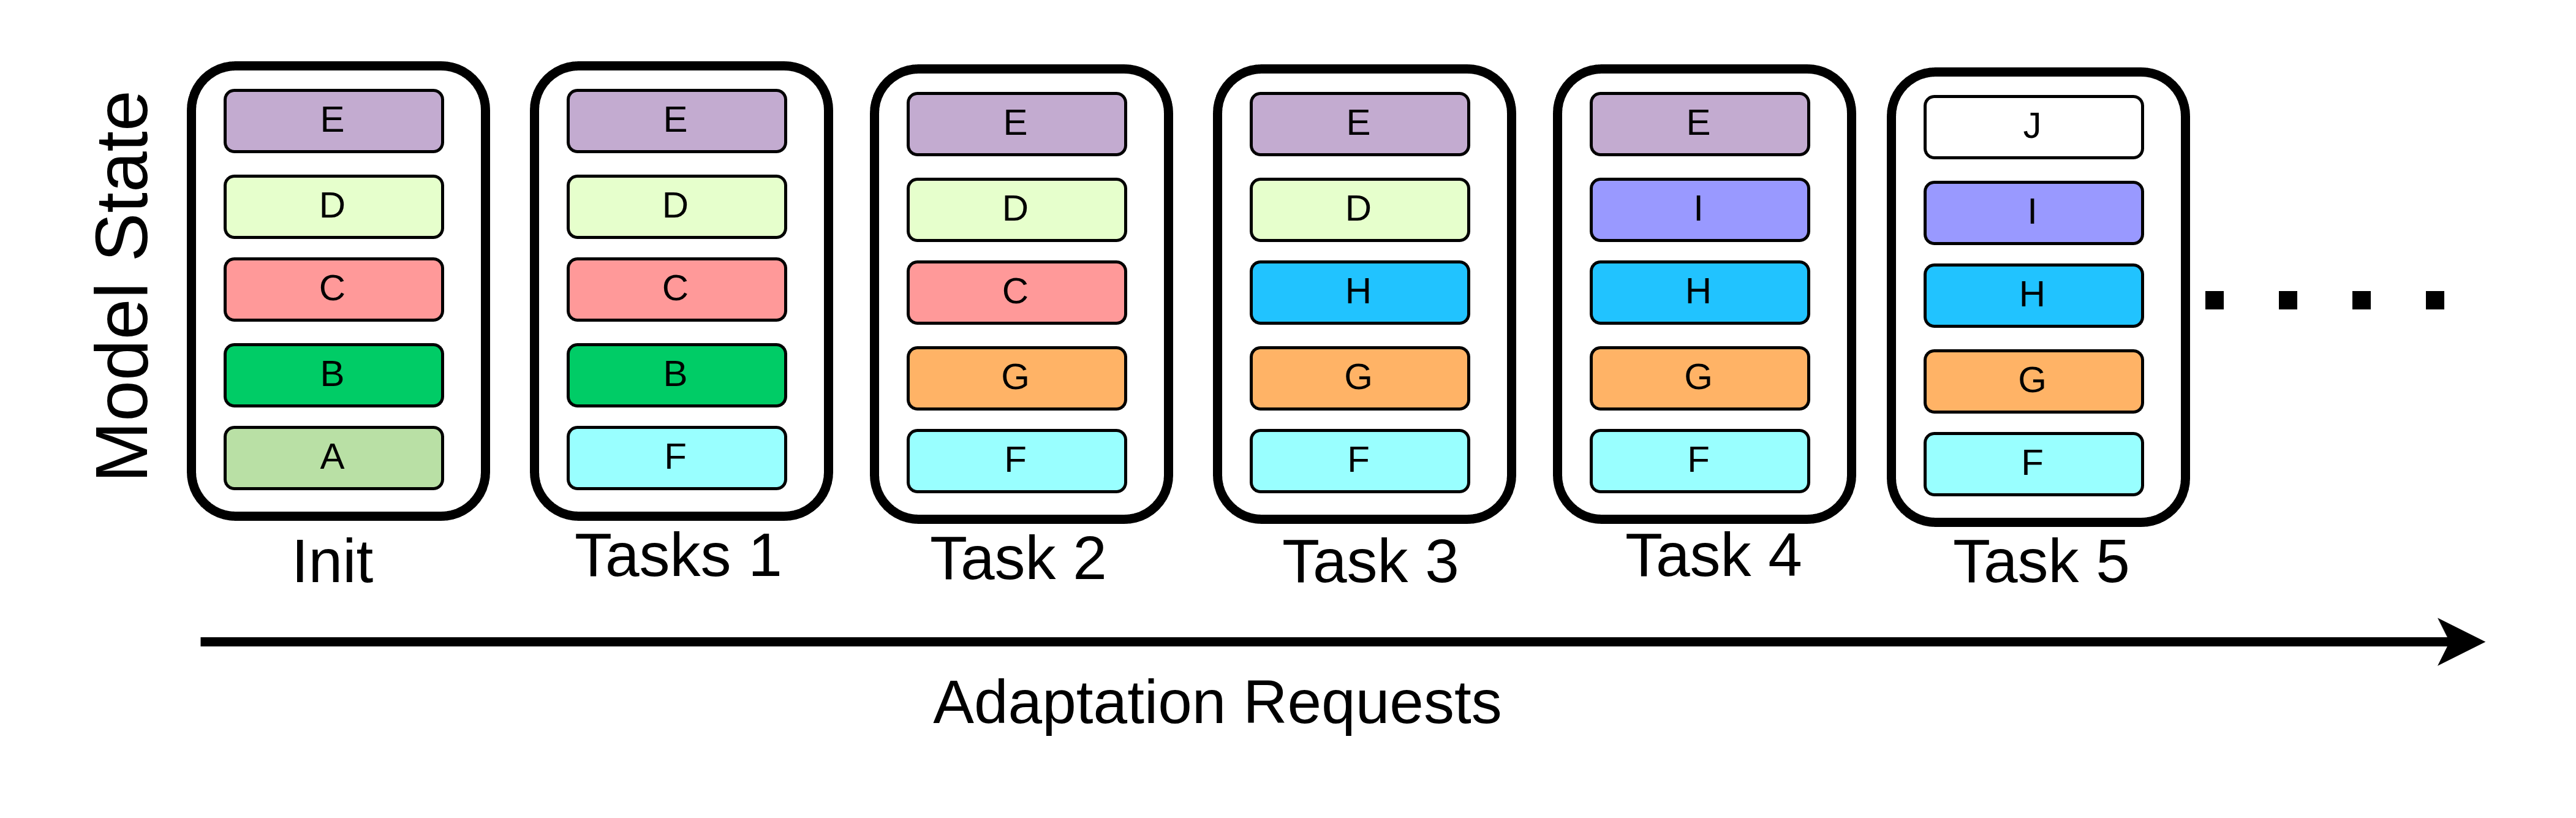
\includegraphics[width=0.75\textwidth]{images/steps.png}
    \caption{Illustration of continual adapting evaluation protocol.}
    \label{fig:sliding_window}
\end{figure}


Ideally, $Acc_f$ should approach zero, while $Acc_r$, $Acc_{n}$, and $Acc_o$ should align with the oracle model's performance. The tunable ratio should approach zero for parameter efficiency. The MIA success rate should approximate 0.5, indicating the adversary cannot distinguish between unlearned and never-seen knowledge. KL divergence should approach zero, indicating no difference at the logit level between the oracle and adapted models.
\subsection{Baseline Implementations}
\label{5.4}

\medskip
\noindent
For baselines, we adopt implementations of existing CLU methods discussed in Section~\ref{2.4}. These include LSF by Shibata et al.~\cite{shibata2021learning}, which introduced the CLU problem and provided an initial solution. We also compare against CLPU-DER++ by Liu et al.~\cite{liu2022continual}, which employs temporal networks for cleaner removal of forget knowledge, UniCLUN by Chatterjee et al.~\cite{chatterjee2024unified}, a student-teacher distillation approach, UnCLe by Adhikari et al.~\cite{adhikari2025unlearning}, which explores hypernetworks for data-free unlearning, and UG-CLU by Huang et al.~\cite{huang2025unified}, a weight saliency-based method.

\subsection{Results Discussion}
\label{5.5}

\medskip
\noindent
Tables~\ref{tab:classification} and~\ref{tab:face_recognition} present results for CIFAR-100 classification and \textcolor{red}{VGGFace2} recognition. BID-LoRA achieves first (\textcolor{green}{green}) or second-best (yellow) performance across nearly all metrics while using only $\approx$ 5.08\% tunable parameters compared to 100\% for all baselines.

\medskip
\noindent
\textit{Unlearning Analysis:} BID-LoRA maintains forget accuracy between 0--0.93\% on CIFAR-100, with 0.93\% in Task 1, 0.27\% in Task 2, and 0.13\% in Task 3, and 0--0.88\% on face recognition, confirming effective unlearning. On CIFAR-100, BID-LoRA achieves the best or second-best overall accuracy in \textcolor{red}{3 of 6} tasks: 76.03\% (Task 1), 76.71\% (Task 4), and 73.51\% (Task 6). \textcolor{red}{MIA and KL divergence results are reported in the ablation study (Section~\ref{7.0}). This parameter efficiency comes with a modest accuracy trade-off: baselines updating 100\% of parameters occasionally match or exceed BID-LoRA's overall accuracy on individual tasks, though at roughly 20\texttimes\ the tunable-parameter cost.}

\medskip
\noindent
\textit{Knowledge Leakage Analysis:} Knowledge leakage, measured by overall accuracy degradation across tasks, remains minimal for BID-LoRA. While baseline methods such as LSF~\cite{shibata2021learning} and UniCLUN~\cite{chatterjee2024unified} show cumulative accuracy drops of 3--8\% from Task 1 to Task 6, BID-LoRA maintains stable performance with only 2.52\% variation on CIFAR-100 (76.03\% $\rightarrow$ 73.51\%) and \textcolor{red}{5.86\% variation on face recognition, ranging from 87.03\% to 92.89\% across Tasks 1--12, demonstrating minimal knowledge leakage despite twice as many adaptation cycles on the larger benchmark. KL divergence results are reported in the ablation study (Section~\ref{7.0}).}

\begin{figure}[!htbp]
    \centering
    \begin{subfigure}[b]{0.38\linewidth}
        \centering
        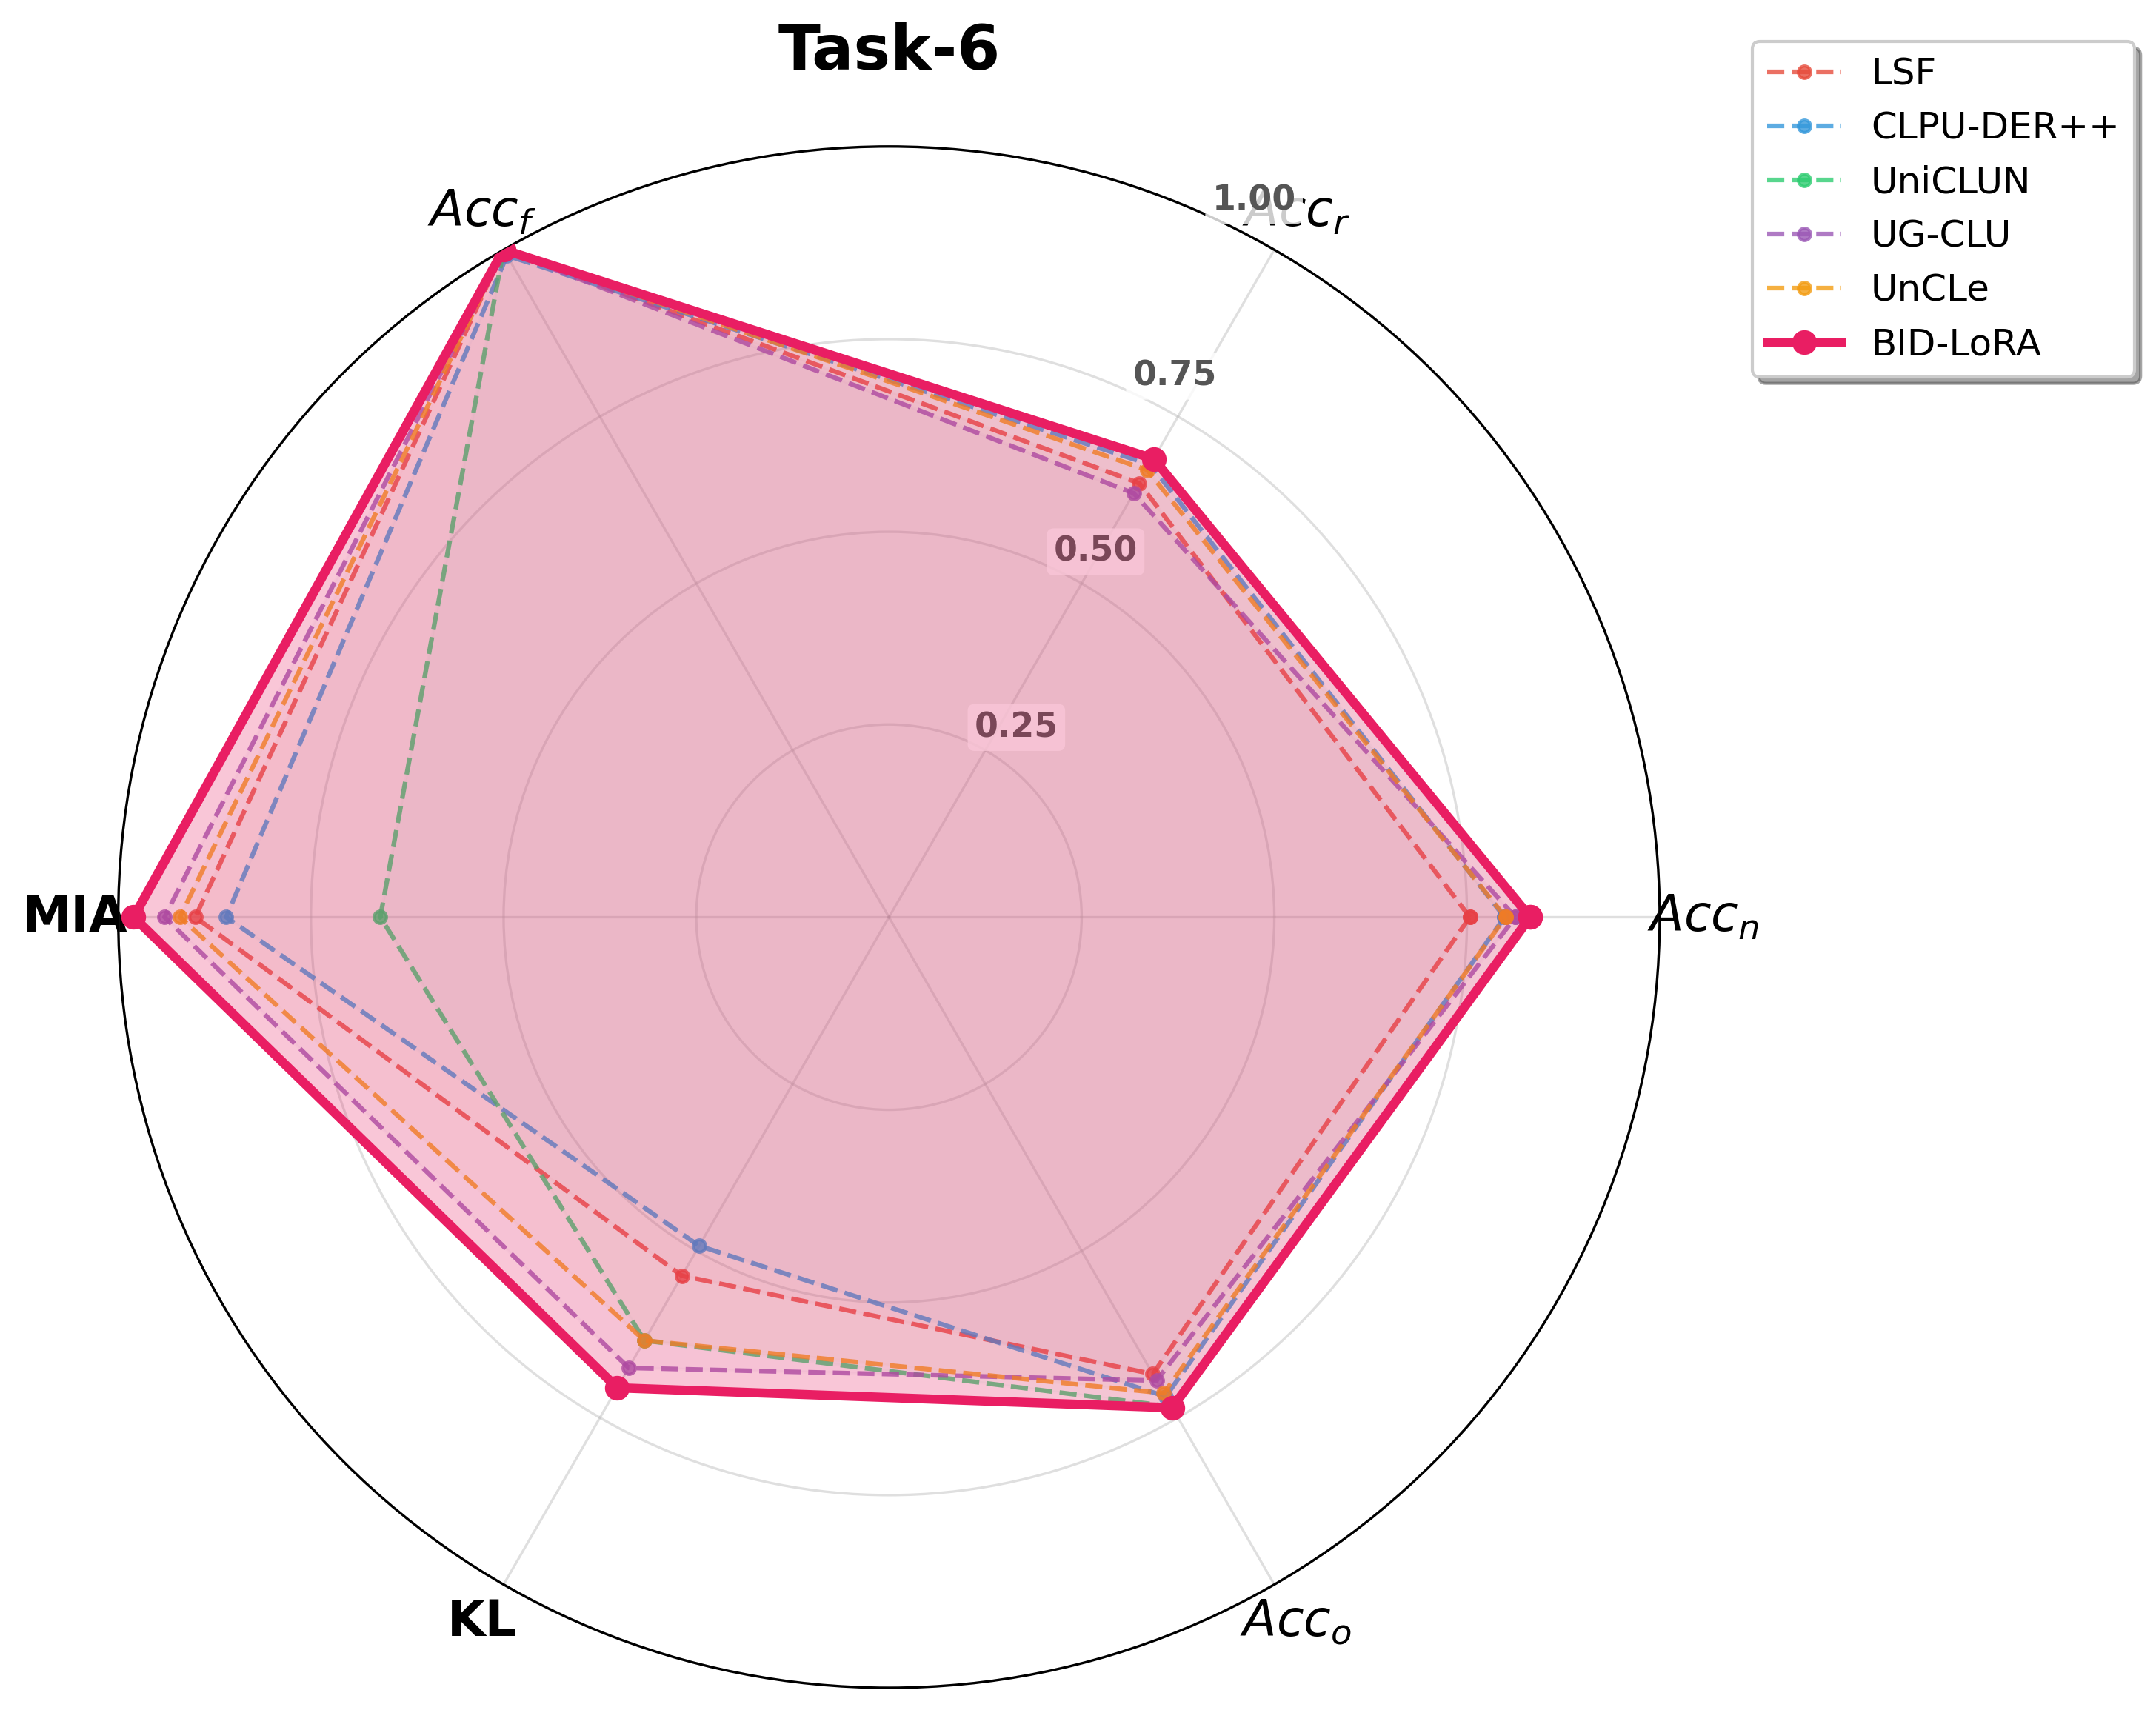
\includegraphics[width=\linewidth]{images/radar_task_6.png}
        \caption{Classification task}
    \end{subfigure}
    \hspace{0.5em}
    \begin{subfigure}[b]{0.38\linewidth}
        \centering
        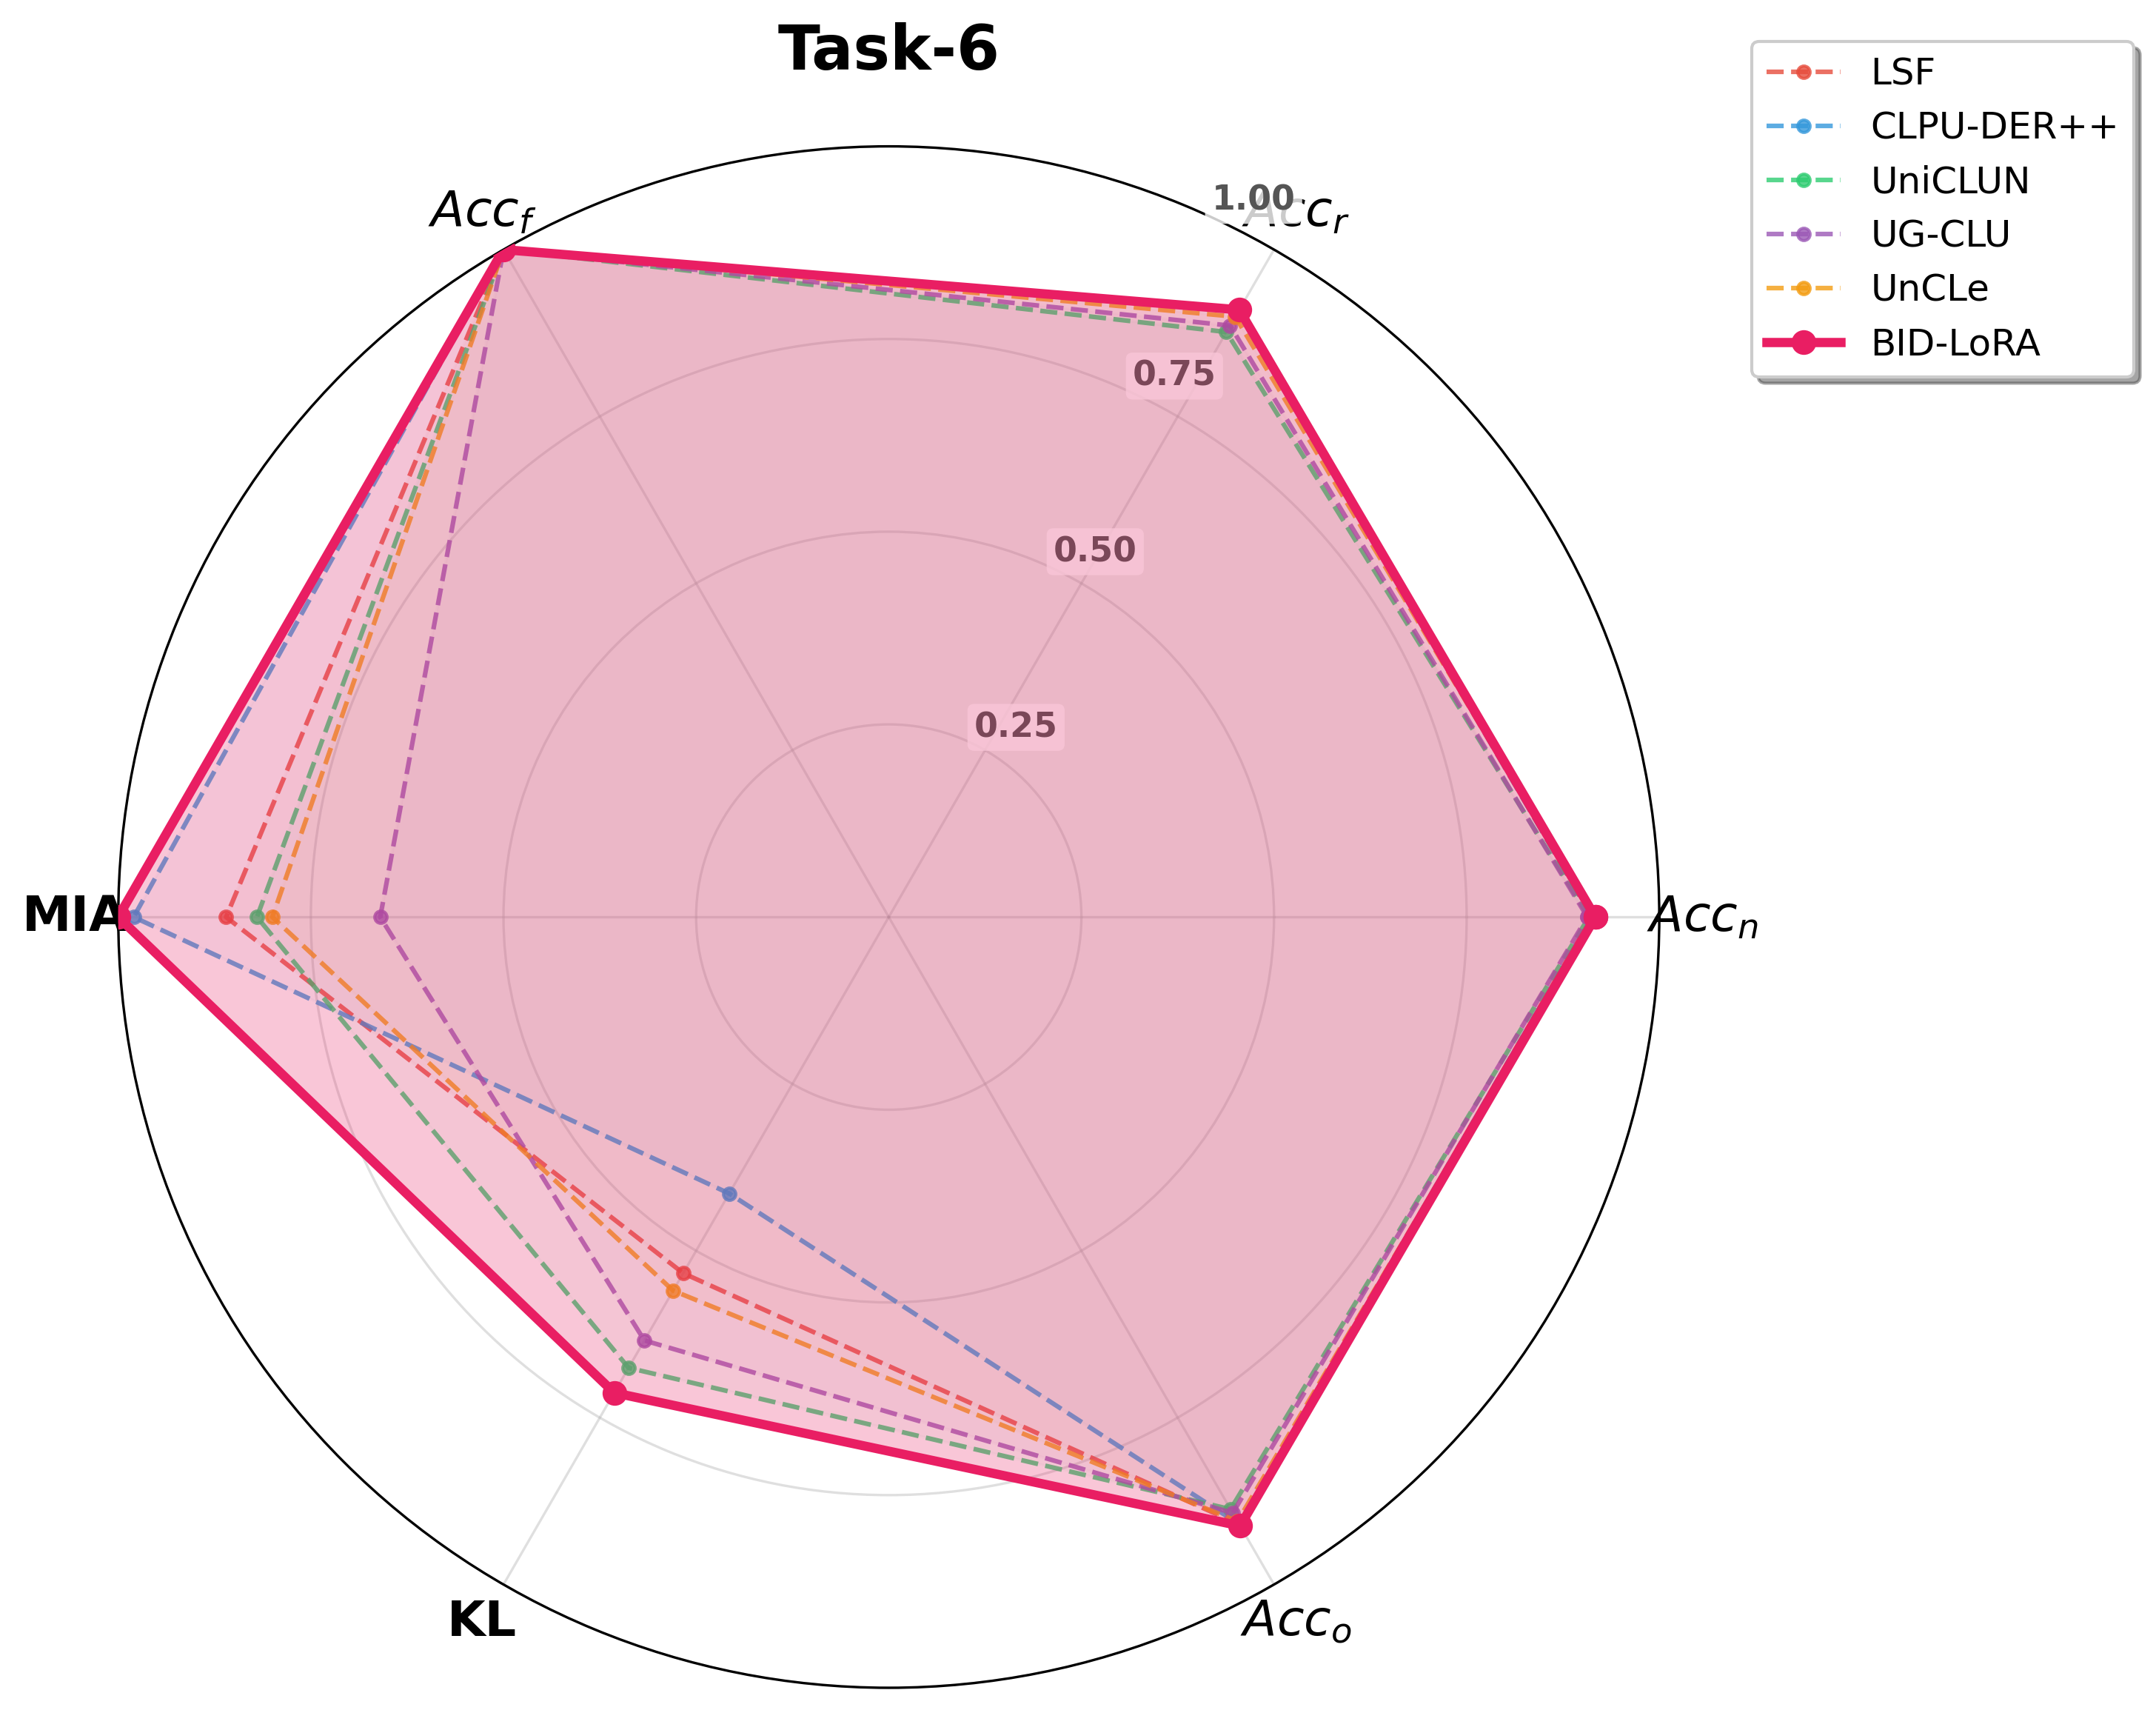
\includegraphics[width=\linewidth]{images/radar_task_6_face.png}
        \caption{Face recognition task}
    \end{subfigure}
    \caption{Radar plot comparison at Task-6. BID-LoRA consistently outperforms all baselines across metrics on both classification and face recognition tasks.}
    \label{fig:radar}
\end{figure}

\medskip
\noindent
\textit{Baseline Comparison:} Combined baseline methods exhibit conflicting optimization between their CL and MU components. LSF~\cite{shibata2021learning} achieves strong unlearning ($Acc_f = 0\%$ in most tasks) but sacrifices overall accuracy, dropping to 68.46\% in Task 6 on CIFAR-100. CLPU-DER++\cite{liu2022continual} and UniCLUN~\cite{chatterjee2024unified} demonstrate unstable retention accuracy, with UniCLUN's $Acc_r$ falling to 67.27\% by Task 2 on CIFAR-100. \textcolor{red}{MIA results for all baselines are reported in the ablation study (Section~\ref{7.0}).} \textcolor{red}{On face recognition, BID-LoRA achieves the best or second-best overall accuracy in 5 of 12 tasks, with $Acc_o$ of 89.69\%, 92.89\%, 92.29\%, 90.50\%, 87.97\%, 91.15\%, 87.03\%, 90.13\%, 89.16\%, 91.92\%, 91.70\%, and 92.61\% across Tasks 1--12 respectively.} As illustrated in Fig~\ref{fig:radar}, BID-LoRA's radar plot at Task-6 encloses all baseline methods, demonstrating superior performance across all evaluation metrics on both classification and face recognition tasks. Similar patterns are observed across CIFAR-100 and \textcolor{red}{VGGFace2} benchmarks.

\medskip
\noindent
\textit{Convergence Patterns:} BID-LoRA exhibits convergent behavior where new knowledge accuracy $Acc_n$ aligns closely with overall accuracy while retained accuracy $Acc_r$ remains stable. On CIFAR-100, new knowledge accuracy $Acc_n$ improves from \textcolor{red}{71.93\% in Task 1 to 80.20\%} in Task 6, while overall accuracy $Acc_o$ remains stable, moving from 76.03\% to 73.51\%, demonstrating effective knowledge acquisition without degrading cumulative performance. Retained accuracy maintains consistency across Tasks 2--6, ranging from \textcolor{red}{68.67\% to 72.33\%}, demonstrating that the bidirectional adapter architecture effectively balances learning and unlearning without catastrophic forgetting.
%\vspace{-0.95cm}
\subsection{Ablation Study}
\label{7.0}
\subsubsection{Parameter Efficiency}
\label{7.1}
We study how LoRA rank affects performance on DeiT-Tiny over 10 epochs. Table~\ref{tab:rank_ablation} shows performance plateaus beyond rank 8, achieving effective adaptation with only $\approx$5\% of parameters versus nearly 100\% for existing methods~\cite{shibata2021learning,adhikari2025unlearning,huang2025unified,chatterjee2024unified,liu2022continual}.
\begin{table}[!htbp]
\centering
\caption{Ablation study on the rank of LoRA modules}
\begin{tabular}{lccccc}
\toprule
Rank & \% Ratio & $Acc_f$ & $Acc_r$ & $Acc_n$ & $Acc_o$ \\
\midrule
1  & 1.09 & 1.73 & 48.57 & 27.60 & 41.58 \\
2  & 2.30 & 3.47 & 46.43 & 43.07 & 45.31 \\
4  & 3.24 & 0.00 & 65.71 & 41.87 & 57.77 \\
\rowcolor{orange!20}
8  & 5.08 & 0.80 & 76.43 & 69.60 & 74.15 \\
16 & 8.56 & 1.07 & 81.43 & 73.73 & 78.86 \\
32 & 14.80 & 0.40 & 78.57 & 76.93 & 78.03 \\
64 & 25.03 & 0.40 & 78.57 & 79.07 & 78.74 \\
\bottomrule
\end{tabular}
\label{tab:rank_ablation}
\end{table}

\subsubsection{BID-LoRA vs Standard LoRA}
\label{7.2}
As discussed in Section~\ref{4}, BID-LoRA employs distinct pathways to handle conflicting tasks like continual learning and unlearning simultaneously. Table~\ref{tab:bid_vs_standard} shows BID-LoRA outperforms standard LoRA (applied to QKV attention and classification head) in the CLU setting over 20 epochs, demonstrating that pathway separation minimizes knowledge leakage between conflicting objectives.

\begin{table}[!htbp]
\centering
\caption{BID-LoRA vs. Standard LoRA in the CLU setting}
\begin{tabular}{lccccc}
\toprule
Method & \% Ratio & $Acc_f$ & $Acc_r$ & $Acc_n$ & $Acc_o$ \\
\midrule
Standard LoRA & 2.54 & 0.00 & 74.29 & 85.07 & 77.88 \\
\rowcolor{orange!20}
BID-LoRA & 5.08 & 0.13 & 77.14 & 85.87 & 80.05 \\
\bottomrule
\end{tabular}
\label{tab:bid_vs_standard}
\end{table}

\subsubsection{Buffer Ratio}
\label{7.3}
Buffer data informs the model what to retain or forget. Here, we examine the effect of retain buffer ratio on overall accuracy. Our method is designed to remain robust even with limited buffer availability, as shown in Table.~\ref{tab:buffer_ratio}.
\begin{table}[!htbp]
\caption{Ablation on retain ratio. \textcolor{red}{$^\dagger$Rel.\ Speedup is the theoretical training-cost reduction (= 1/retain ratio), assuming cost scales linearly with buffer size; it is not a measured wall-clock time.}}
\centering
\begin{tabular}{lccccc}
\toprule
Retain Ratio & \textcolor{red}{Rel.\ Speedup$^\dagger$} & $Acc_f$ & $Acc_r$ & $Acc_n$ & $Acc_o$ \\
\midrule
1.0 & 1.0$\times$ & 0.40 & 68.00 & 81.74 & 72.58 \\
0.5 & 2.0$\times$ & 0.00 & 70.00 & 71.05 & 70.35 \\
0.3 & 3.3$\times$ & 0.00 & 66.00 & 79.11 & 70.37 \\
\rowcolor{orange!20}
0.1 & 10$\times$ & 0.00 & 65.00 & 79.96 & 69.98 \\
\bottomrule
\end{tabular}
\label{tab:buffer_ratio}
\end{table}
%\vspace{-0.74cm}
\subsubsection{Ablation on Adapters}
\label{7.4}


\begin{table}[!htbp]
\caption{Ablation on adapter pathway contributions (F=Forget, R=Retain, N=New)}
\centering
\begin{tabular}{ccc|cccc}
\toprule
F & R & N & $Acc_f$ & $Acc_r$ & $Acc_n$ & $Acc_o$ \\
\midrule
\multicolumn{3}{c|}{Pre-train} & 73.64 & 82.27 & 0.00 & 48.49 \\
\midrule
\xmark & \cmark & \cmark & 70.45 & 82.73 & 51.82 & 72.43 \\
\cmark & \xmark & \cmark & 0.00 & 0.23 & 64.55 & 21.67 \\
\rowcolor{orange!20}
\cmark & \cmark & \cmark & 0.00 & 84.09 & 56.82 & 75.00 \\
\cmark & \cmark & \xmark & 0.00 & 84.09 & 0.00 & 56.06 \\
\bottomrule
\end{tabular}
\label{tab:adapter_ablation}
\end{table}


This experiment verifies that each adapter pathway holds knowledge specific to its task. By selectively disabling pathways, we observe accuracy drops for retain and new tasks, while forget accuracy increases when its pathway is disabled. As shown in Table~\ref{tab:adapter_ablation}, the optimal performance is achieved only when all three pathways are active, validating the necessity of the tri-pathway architecture. The original classification head is restored during evaluation to isolate adapter contributions. Results are obtained over 15 epochs with pathways disabled during testing.

\subsubsection{Geometric Verification of Unlearning}
\label{7.5}
A critical question is whether forget-class embeddings actually move toward the computed escape direction $d^*$. Fig ~\ref{fig:geometric_verification}(a,b) shows t-SNE visualizations before and after unlearning. Initially, the three forget classes (0, 1, 2) are spatially separated from $d^*$. After unlearning, all three forget clusters collapse toward the dustbin point, demonstrating successful alignment with the intended escape direction.
The 3D sphere visualizations (Fig ~\ref{fig:geometric_verification} (c,d)) provide additional evidence by showing class centroids projected onto a unit sphere via PCA. While retain-class centroids (R3--R9, squares) remain anchored at their original positions relative to the retain centroid $\bar{c}_r$, the forget centroids (F0, F1, F2, circles) migrate along the antipodal axis toward $d^*$. Notably, F1 moves from a position distant from $d^*$ to near-perfect alignment after unlearning, while F0 and F2 also show substantial movement toward the escape direction. This confirms that the optimization successfully drives forget-class representations away from retain classes along the computed global escape vector.


\begin{figure}[!htbp]
    \centering
    \begin{subfigure}[b]{0.38\linewidth}
        \centering
        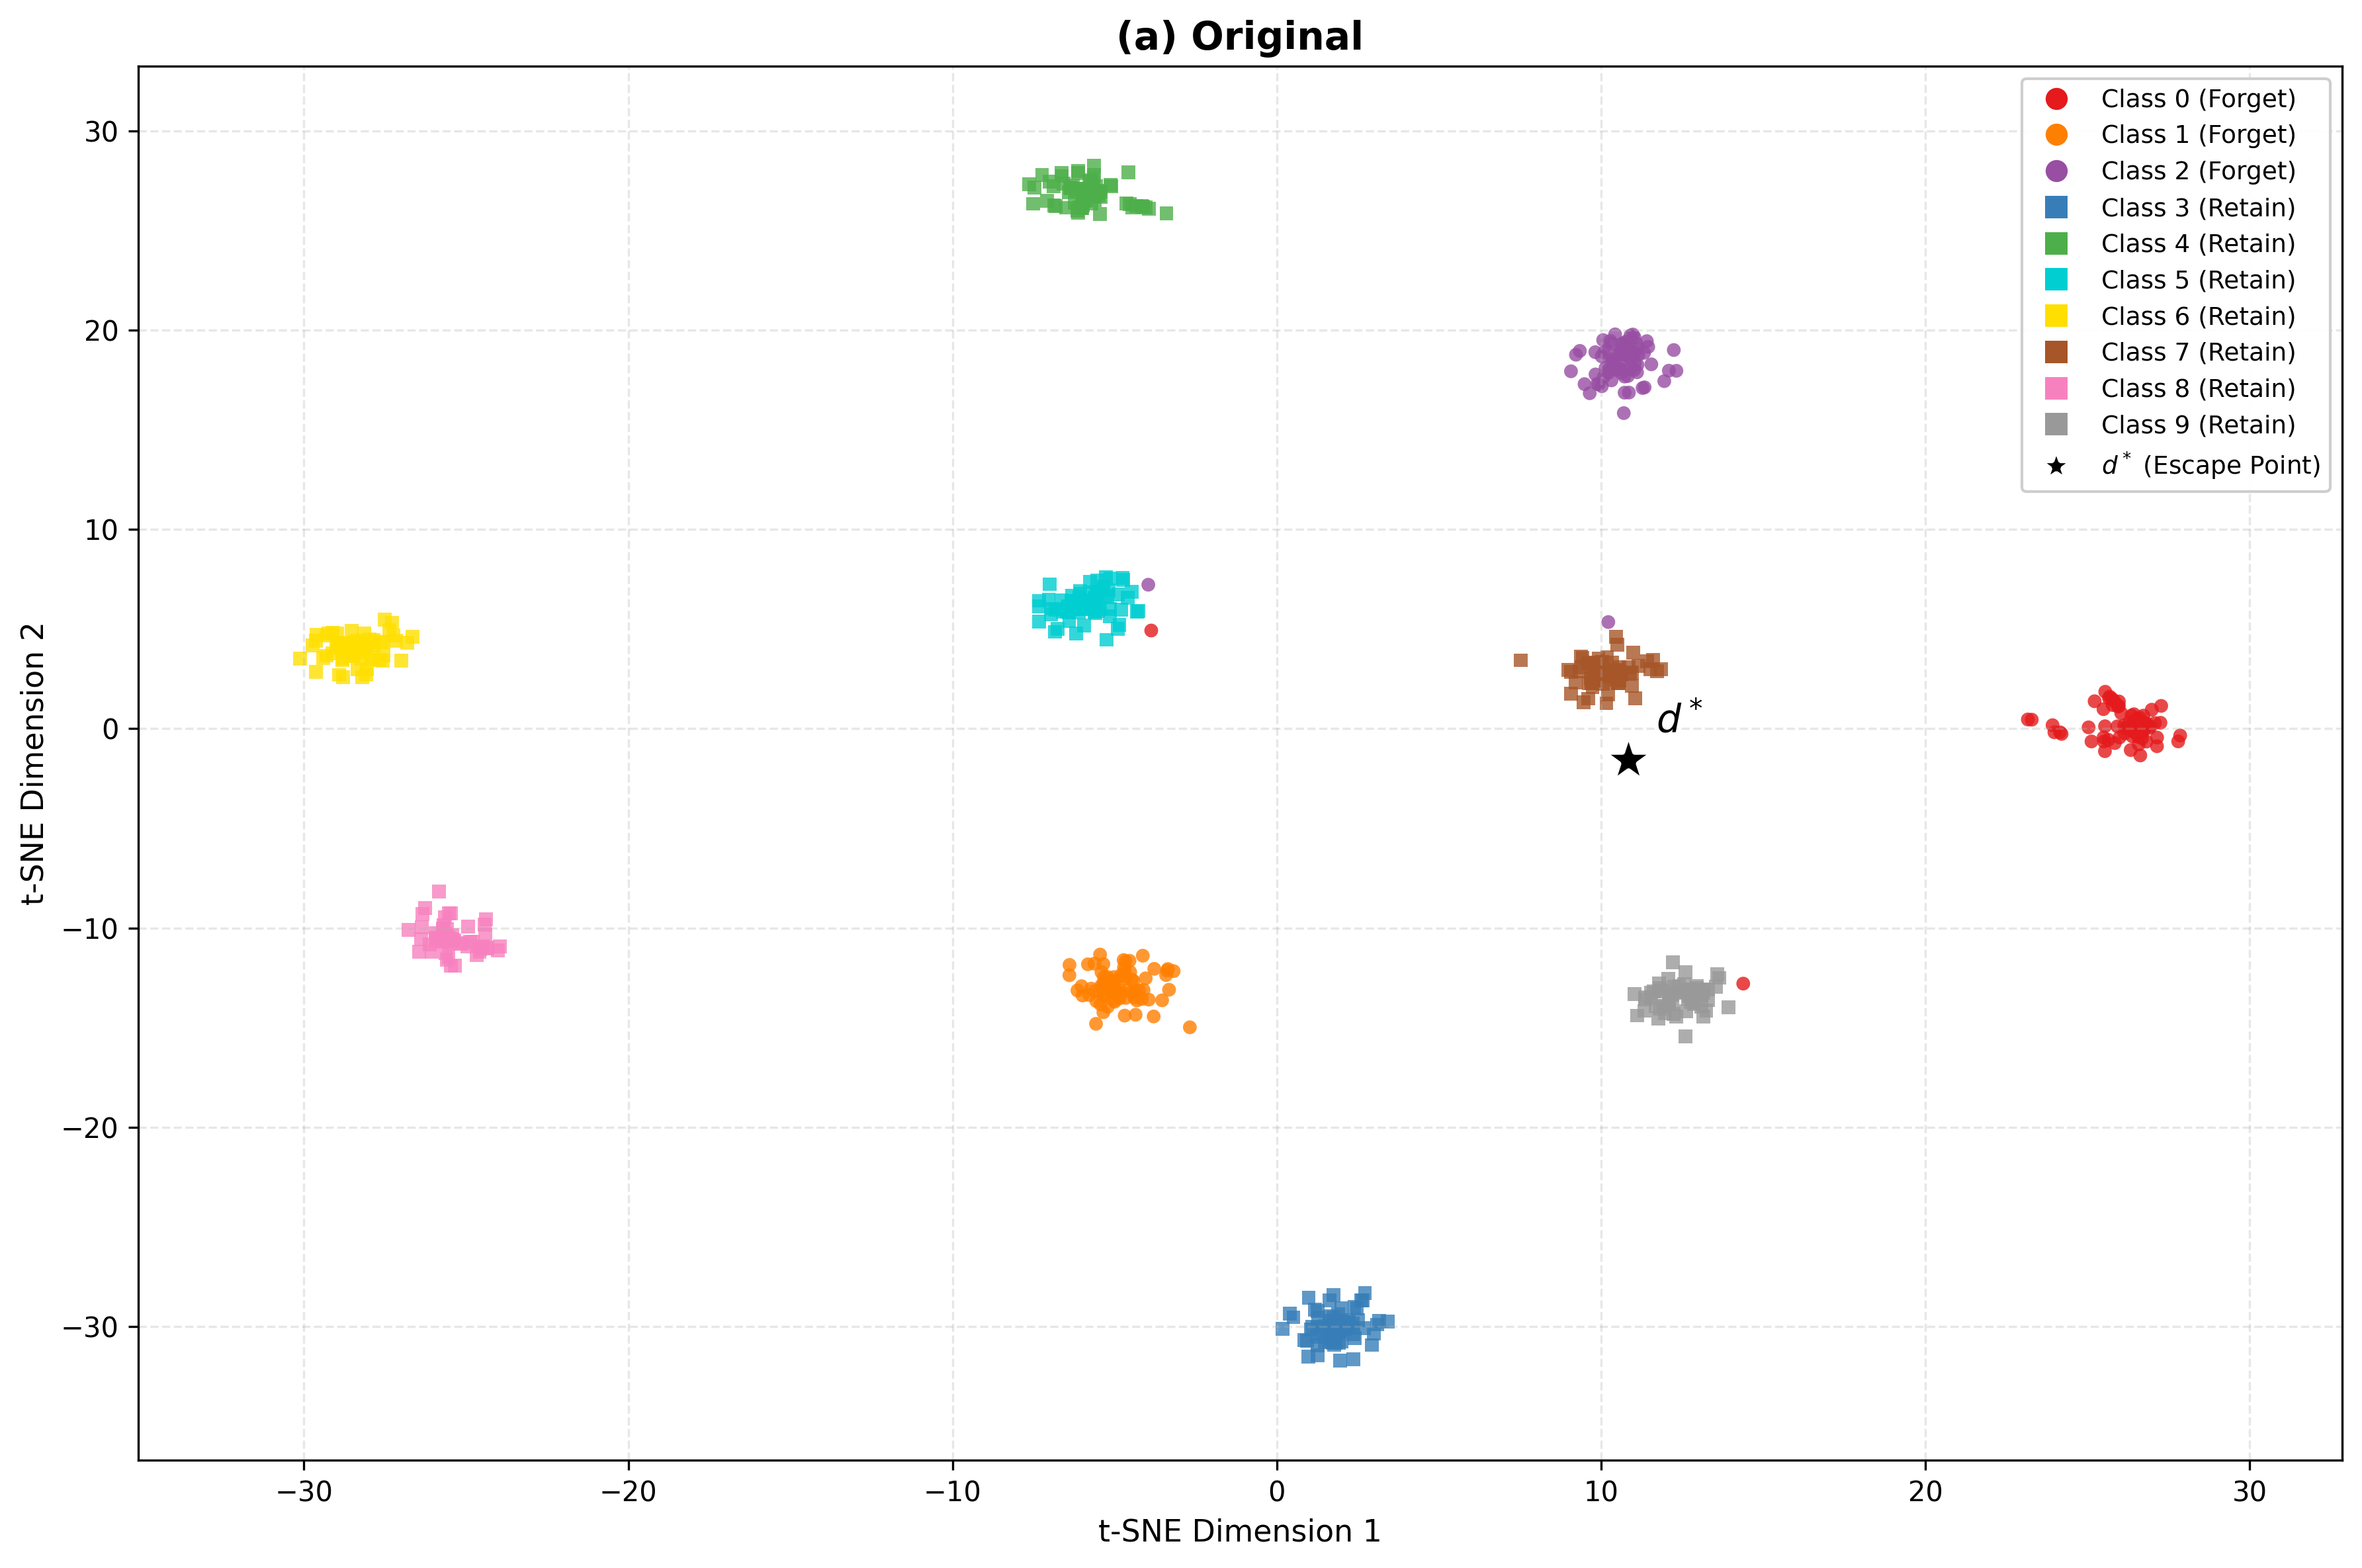
\includegraphics[width=\linewidth]{images/tsne_epoch_00.png}
        \caption{t-SNE: Before unlearning}
    \end{subfigure}
    \hspace{0.5em}
    \begin{subfigure}[b]{0.38\linewidth}
        \centering
        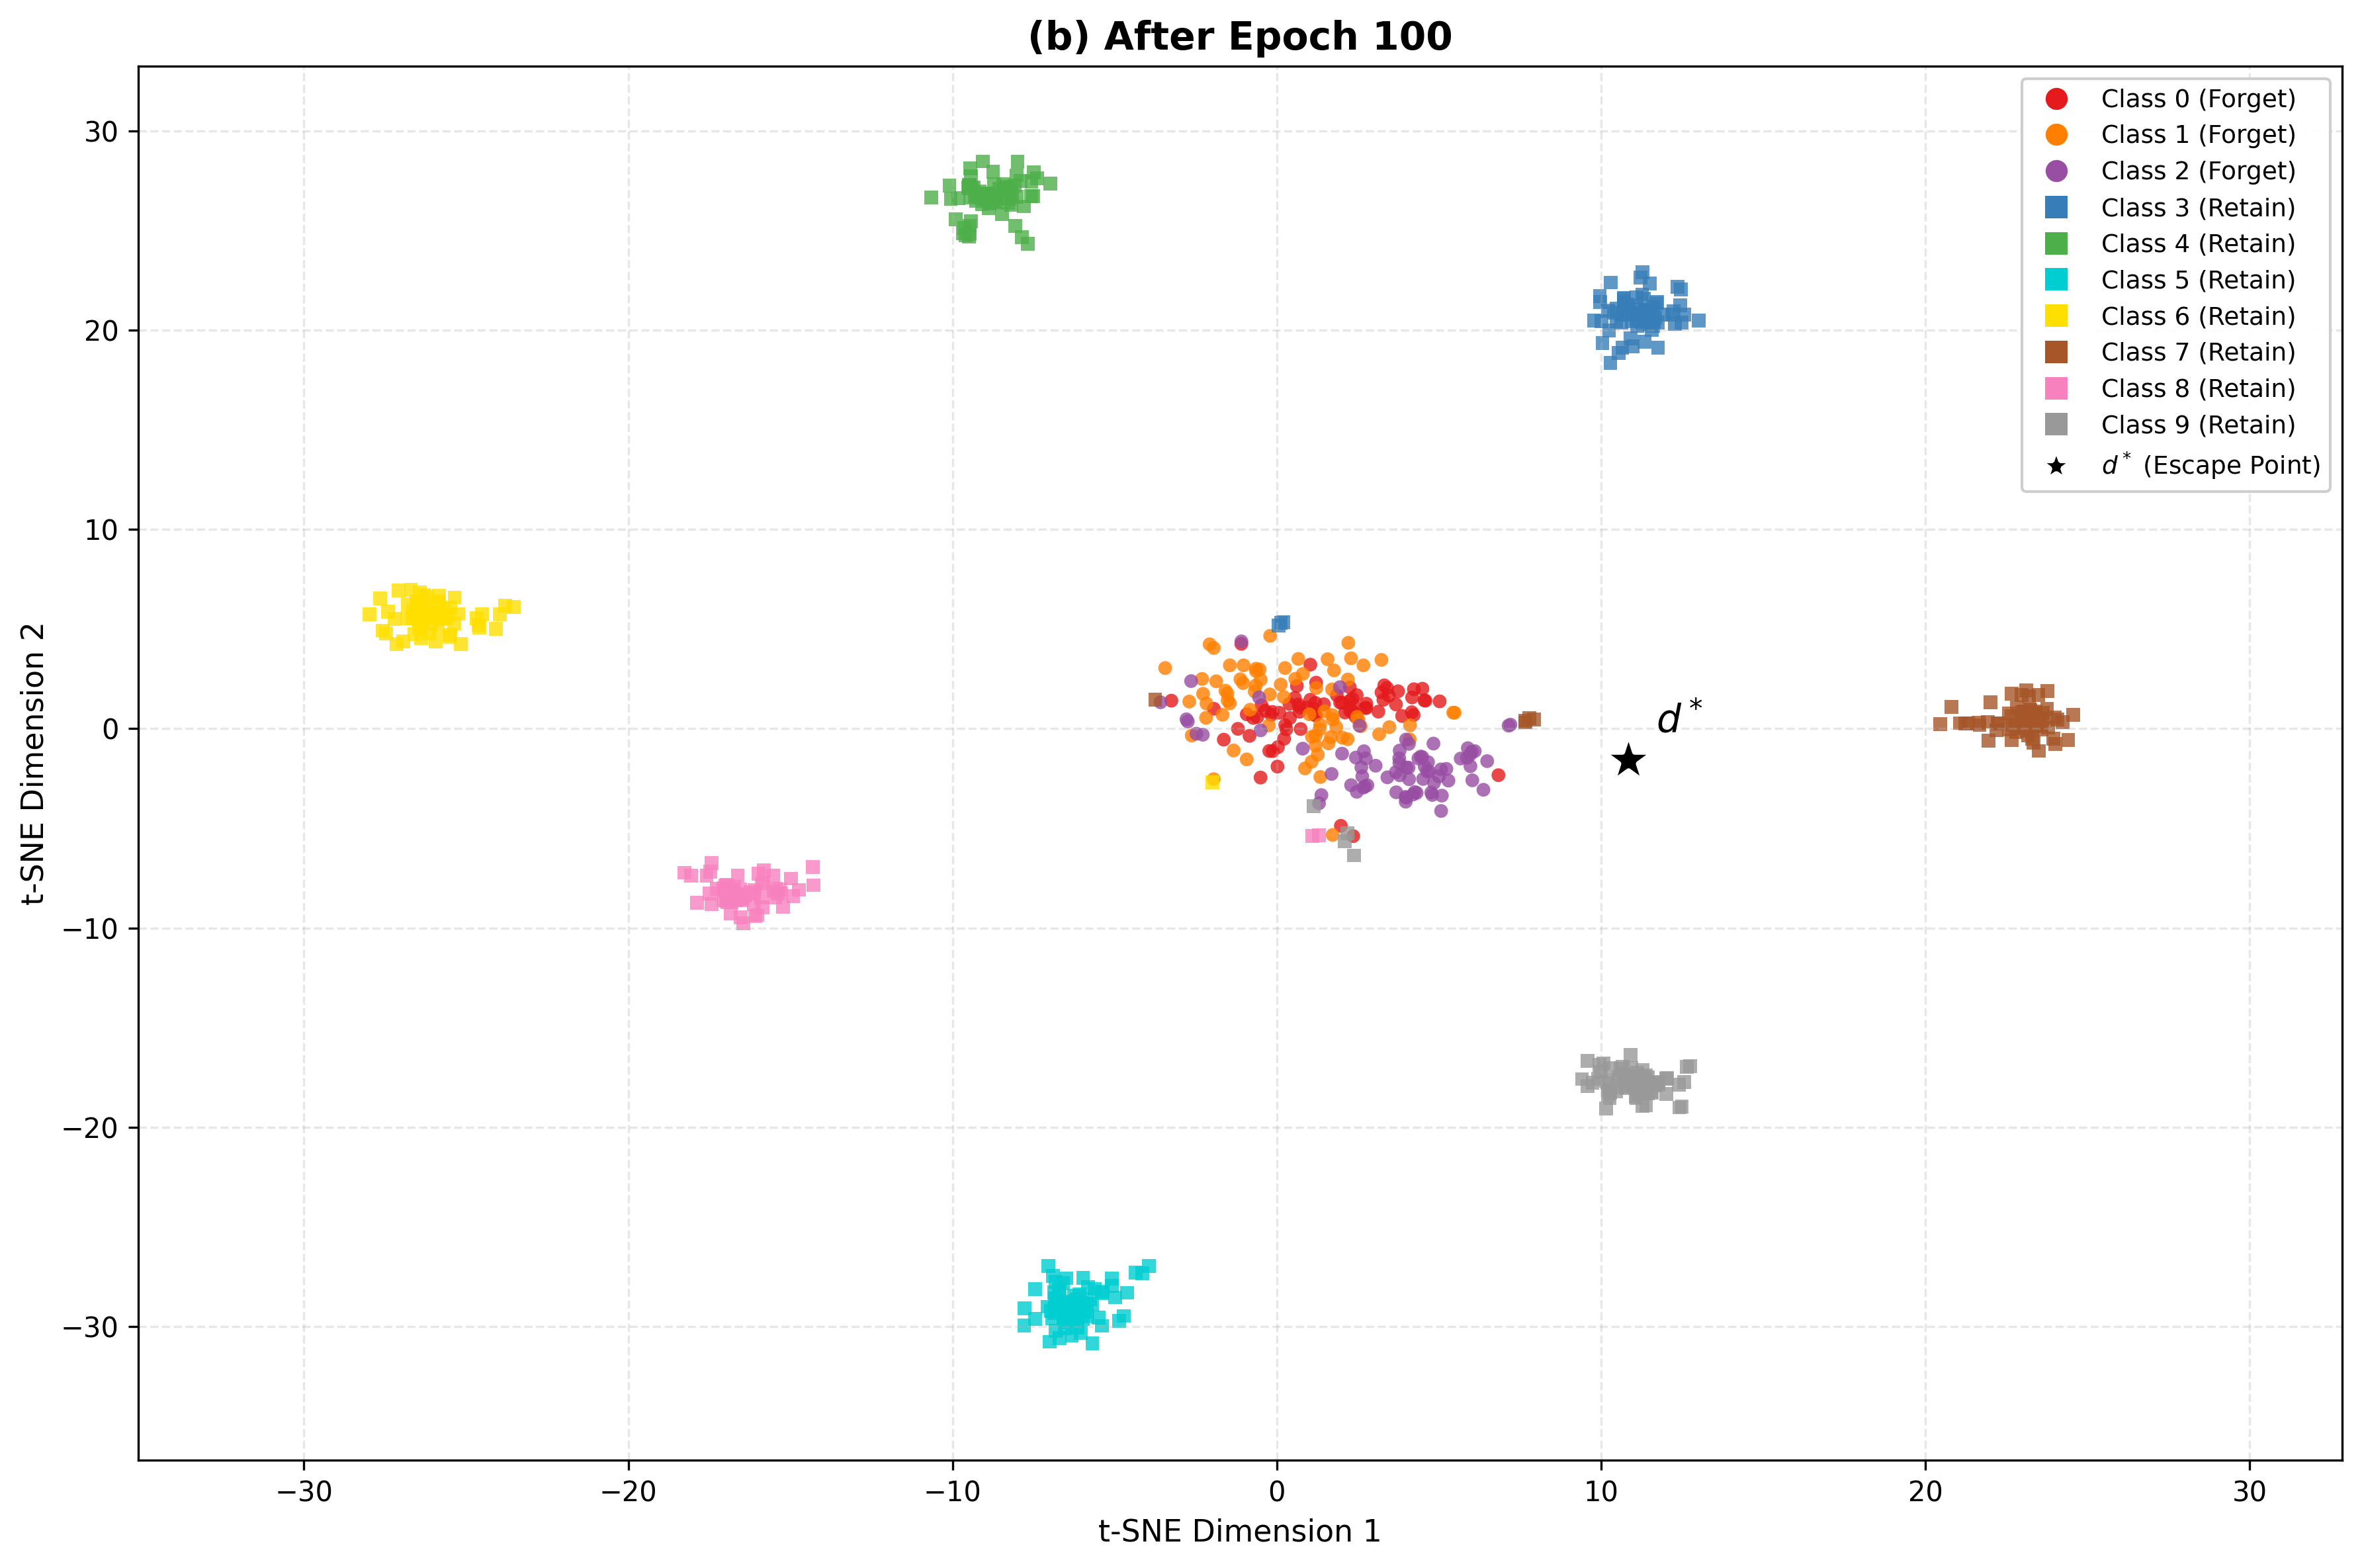
\includegraphics[width=\linewidth]{images/tsne_epoch_100.png}
        \caption{t-SNE: After unlearning}
    \end{subfigure}

    \vspace{0.8em}

    \begin{subfigure}[b]{0.38\linewidth}
        \centering
        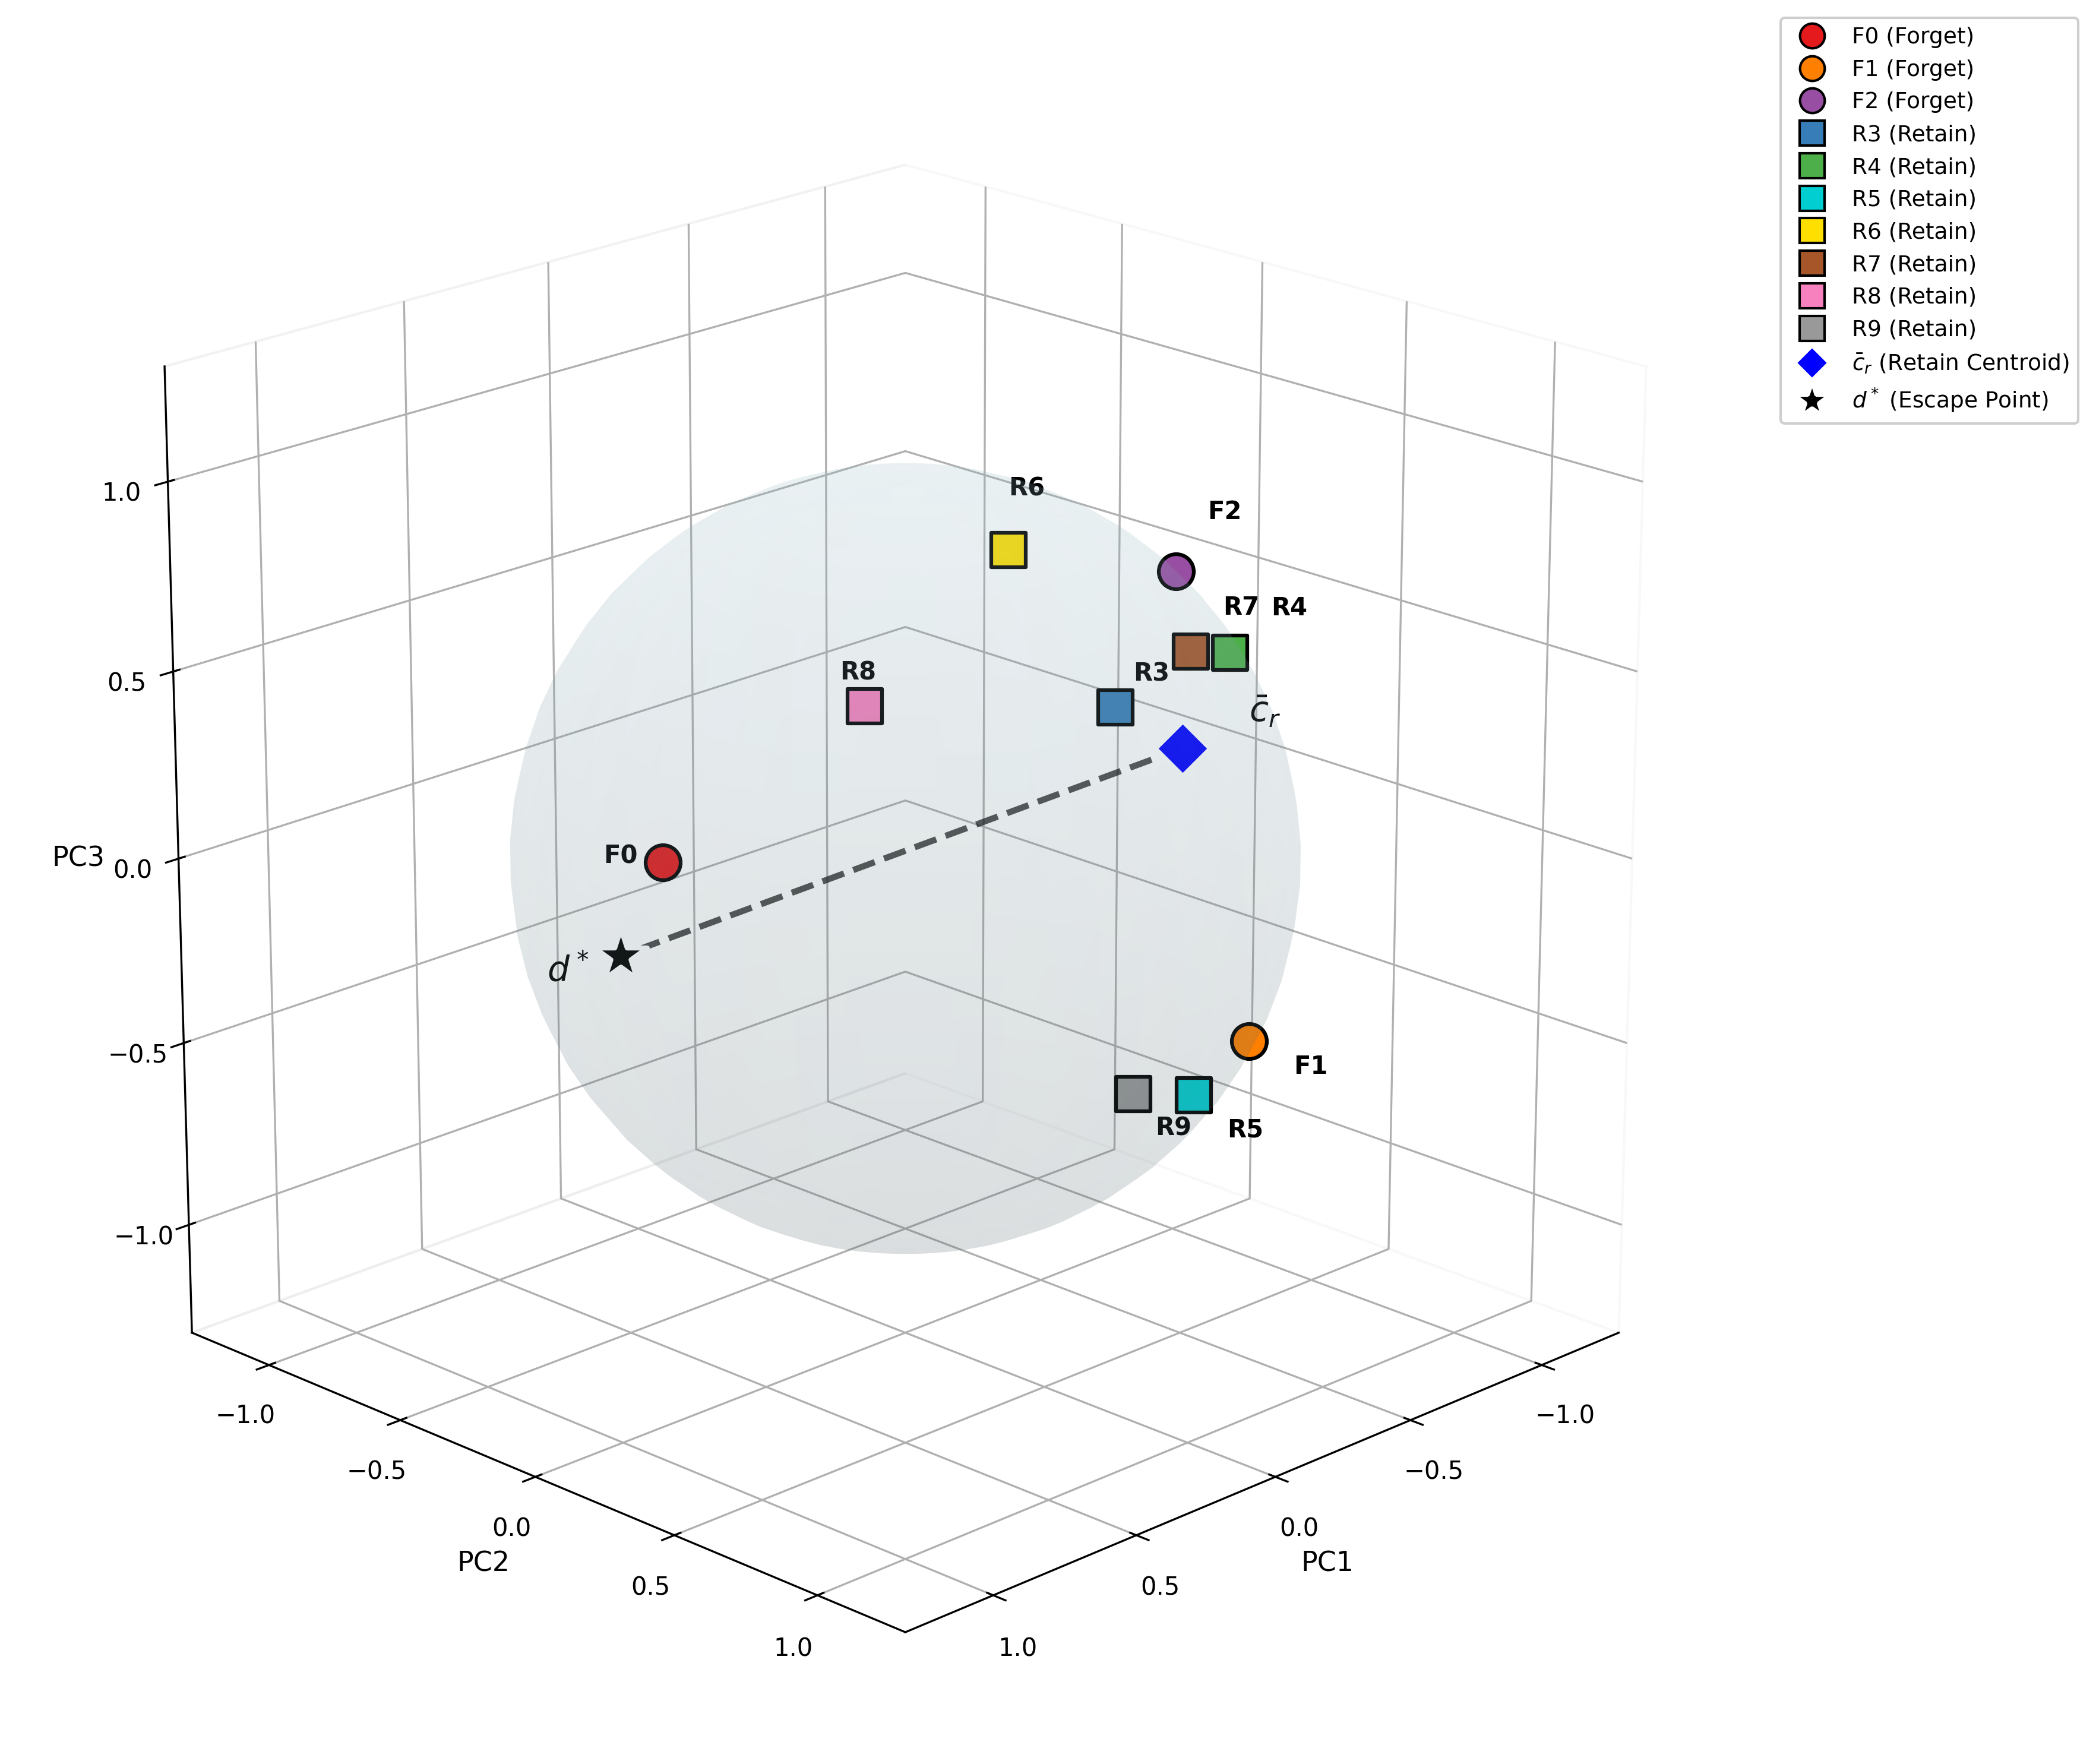
\includegraphics[width=\linewidth]{images/sphere_centroid_00.png}
        \caption{3D sphere: Before unlearning}
    \end{subfigure}
    \hspace{0.5em}
    \begin{subfigure}[b]{0.38\linewidth}
        \centering
        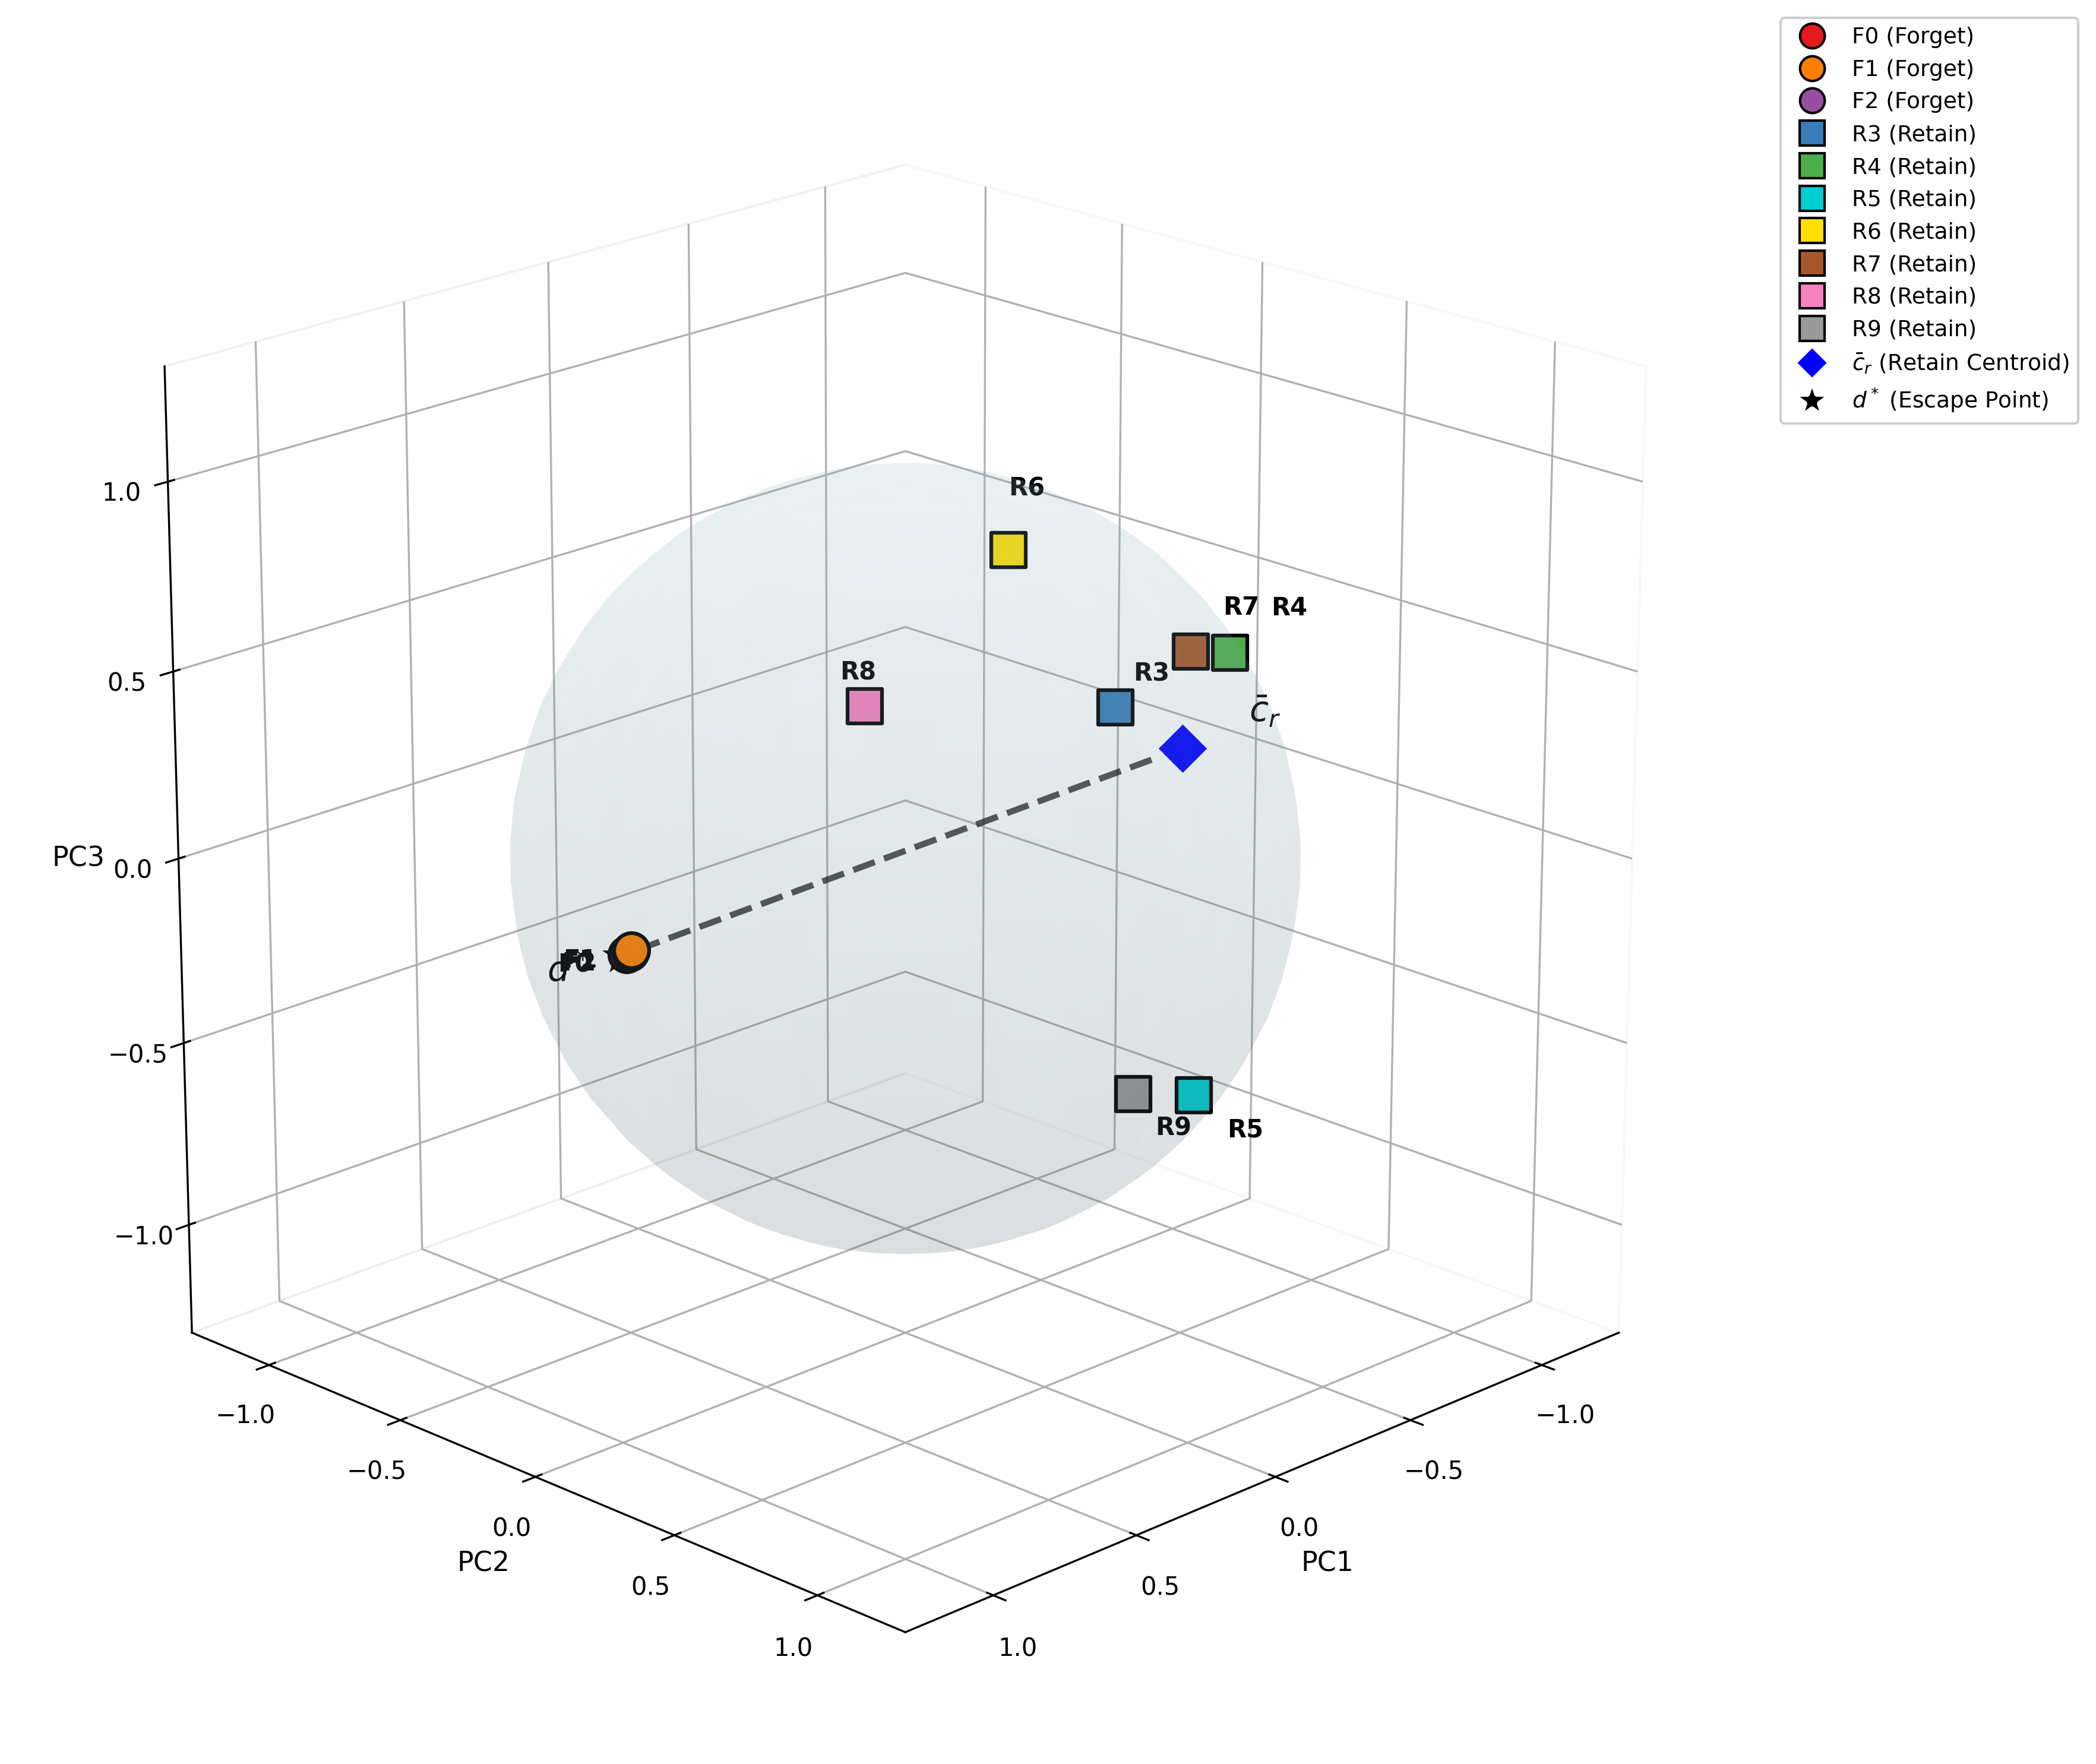
\includegraphics[width=\linewidth]{images/sphere_centroid_18.png}
        \caption{3D sphere: After unlearning}
    \end{subfigure}

    \caption{Geometric verification of unlearning. Top row: t-SNE visualization showing forget classes migrating toward escape point $d^*$. Bottom row: 3D hypersphere visualization with dashed antipodal axis from $\bar{c}_r$ to $d^*$.}
    \label{fig:geometric_verification}
\end{figure}



\subsubsection{Escape Point Scaling}
\label{7.6}
As discussed in Section~\ref{4.3}, placing $d^*$ on the unit sphere leads to unstable forgetting due to nearby centroids. Table~\ref{tab:escape_ablation} validates this: $\lambda_{\text{esc}}=10$ achieves optimal forgetting (0.53\%) by pushing the escape point beyond the embedding sphere.


% =====================================================================
% !!! PLACEHOLDER NUMBERS in tab:unlearning_evidence -- DRAFT SKELETON.
% Every value is ASSUMED. Replace with measured results before
% submission. The paragraph underneath asserts three of them
% qualitatively (Sink high, probe below Oracle, relearn ~= Oracle):
% re-check it if the measurements come out differently.
% =====================================================================

\subsubsection{\textcolor{red}{Unlearning Evidence Under Attack}}
\label{7.7}

\begin{table}[!htbp]
\centering
\footnotesize
\caption{\textcolor{red}{Unlearning evidence under attack, on the Task-6 CIFAR-100 checkpoint over all 60 classes forgotten during Tasks 1--6.}}
\label{tab:unlearning_evidence}
\textcolor{red}{
\begin{tabular}{lccc}
\toprule
\textbf{Evaluation} & \textbf{Original} & \textbf{BID-LoRA} & \textbf{Oracle} \\
                    & \textbf{(no unlearning)} & \textbf{(ours)} & \textbf{(retrain)} \\
\midrule
\multicolumn{4}{l}{\textit{Forgetting holds}} \\
\quad $Acc_f$ (cumulative, all 60 forgotten classes) $\downarrow$ & 72.91 & \textbf{0.00} & -- \\
\quad Sink: share in dominant wrong class & 4.20 & 71.34 & 14.68 \\
\midrule
\multicolumn{4}{l}{\textit{Is the information still there?}} \\
\quad Linear probe on frozen emb. (forget-class ID) $\downarrow$ & 68.53 & \textbf{8.41} & 24.77 \\
\quad Relearn @ 5-shot $\rightarrow Acc_f$ $\downarrow$ & 74.30 & \textbf{19.72} & 23.41 \\
\quad Relearn: epochs to 50\% of original $Acc_f$ $\uparrow$ & 0 & \textbf{$>$50} & $>$50 \\
\midrule
\multicolumn{4}{l}{\textit{Privacy attacks}} \\
\quad MIA, confidence-based $\approx 0.5$ & 0.78 & \textbf{0.51} & 0.50 \\
\quad MIA, label-only~\cite{choquette2021label} $\approx 0.5$ & 0.71 & \textbf{0.52} & 0.51 \\
\quad MIA, adaptive (distance to $t_{\text{escape}}$) $\approx 0.5$ & 0.50 & \textbf{0.53} & 0.50 \\
\quad Model inversion: identity match rate $\downarrow$ & 61.20 & \textbf{3.74} & 4.11 \\
\midrule
\multicolumn{4}{l}{\textit{Oracle consistency}} \\
\quad Prediction agreement with Oracle on $D_f$ $\uparrow$ & 0.12 & \textbf{0.88} & 1.00 \\
\quad KL divergence vs.\ Oracle $\downarrow$ & 3.41 & \textbf{0.79} & 0.00 \\
\bottomrule
\end{tabular}
}
\end{table}

\textcolor{red}{\emph{Original} is the pre-adaptation model and \emph{Oracle} is retrained from scratch without $D_f$, so the two bracket each attack: information present versus absent by construction. The Oracle column, not $0.5$, is therefore the target for every row, and BID-LoRA matches it on all eleven measurements. The high Sink with a probe below Oracle (chance $1/60=1.67\%$) shows collapse, not relabelling; 5-shot relearning recovers no faster than from scratch, which is what we mean by irreversible. All three MIAs use a 3-layer MLP over per-sample loss and confidence features, 5 attack initialisations, and balanced sets of 200 samples per class, with non-members drawn from held-out images of the same forgotten classes; the adaptive variant instead thresholds $\lVert \text{emb}(x)-t_{\text{escape}} \rVert$. Model inversion additionally covers class-prototype extraction, as the two share a procedure. These are empirical, attack-relative results, not a formal guarantee.}

\section{Discussion}
\label{8.0}
In this section, we provide an in-depth discussion of several critical aspects of our approach. We examine the theoretical necessity of retain data in machine unlearning, present an algorithmic perspective of our BID-LoRA method, and analyze the knowledge leakage phenomenon that motivates our unified framework. These discussions provide deeper insights into the design principles and empirical observations underlying our work.
\vspace{0.0cm}
\subsection{On the Necessity of Retain Buffer in Machine Unlearning}
\label{8.1}
Effective unlearning requires distinguishing what to forget from what to retain. This section investigates whether forget data ($D_f$) or retain buffer ($D_r$, a subset of full retain data $D^\text{full}_r$) can be avoided in classification and face recognition tasks.

We find $D_r$ is fundamentally unavoidable for preserving task-critical knowledge. Without architectural support (e.g., modular pathways), all parameters are adjusted using both $D_f$ and $D^\text{full}_r$ during pretraining, making disentanglement infeasible without $D_r$ access.


\begin{table}[!htbp]
\centering
\caption{Ablation on escape scaling factor $\lambda_{\text{esc}}$. Higher scaling pushes forget embeddings further from retain centroids, improving unlearning}
\begin{tabular}{ccccc}
\toprule
$\lambda_{\text{esc}}$ & $Acc_f \downarrow$ & $Acc_r \uparrow$ & $Acc_n \uparrow$ & $Acc_o \uparrow$ \\
\midrule
0 & 8.80 & 78.57 & 61.07 & 72.74 \\
2 & 4.13 & 80.71 & 63.60 & 75.01 \\
5 & 4.27 & 77.14 & 68.27 & 74.18 \\
\rowcolor{orange!15}
10 & 0.53 & 77.14 & 68.00 & 73.45 \\
\bottomrule
\end{tabular}
\label{tab:escape_ablation}
\end{table}


Only noise-based impair-and-repair methods~\cite{tarun2023fast} and source-free unlearning~\cite{ahmed2025towards} attempt to bypass data dependencies. The former still requires $D_r$. Source-free methods estimate retain data Hessians using only $D_f$ through semi-definite programming, but are limited to convex losses and linear classifiers, making them inapplicable to modern non-convex architectures like transformers and ResNets. In practice, they use frozen pre-trained feature extractors and unlearn only linear heads. While error bounds improve with dimensionality, Hessian storage and inversion become computationally prohibitive.

All established methods for non-convex models critically rely on $D_r$. Weight-importance methods (EWC~\cite{kirkpatrick2017overcoming}, SALUN~\cite{fan2023salun}) compute Fisher information or saliency from $D_r$ to protect retain-relevant weights. SCRUB~\cite{kurmanji2023towards} and GS-LoRA~\cite{zhao2024continual} explicitly leverage $D_r$ to safeguard retained knowledge. CLU methods universally depend on $D_r$: LSF~\cite{shibata2021learning} uses mnemonic codes, UnCLe~\cite{adhikari2025unlearning} employs task embeddings, CLPU-DER++~\cite{liu2022continual} maintains experience replay, and UniCLUN~\cite{chatterjee2024unified} and UG-CLU~\cite{huang2025unified} incorporate $D_r$ for stability.

Generative tasks present exceptions: FLAT~\cite{wang2024llm} solves unlearning without $D_r$ through regularizers, while ESD~\cite{gandikota2023erasing} avoids both $D_f$ and $D_r$ using teacher models to generate synthetic samples.

While $D_f$ can theoretically be avoided through noise-based proxies or source-free methods, no viable approach eliminates $D_r$ dependence for non-convex deep learning without compromising retention performance.

\subsection{Knowledge Leakage Analysis}
\label{8.2}

Can we solve CLU by combining existing CL and MU methods? We pair four combinations (ER-ACE\cite{caccia2021new} + GS\cite{zhao2024continual} ), (DER++ \cite{buzzega2020dark} + FU \cite{tarun2023fast}), (EWC \cite{kirkpatrick2017overcoming} + SalUn\cite{fan2023salun}), and (ER-AML \cite{caccia2021new} + GS\cite{zhao2024continual}) on data-efficient image transformers~\cite{touvron2021training} and FaceTransformer~\cite{zhong2021face} (face recognition). As shown in Fig~\ref{fig:pilot_study}, all exhibit progressive knowledge leakage across CLU cycles, confirming that piecewise solutions fail and a unified framework is necessary.

\begin{figure}[!htbp]
    \centering
    \begin{subfigure}[b]{0.38\linewidth}
        \centering
        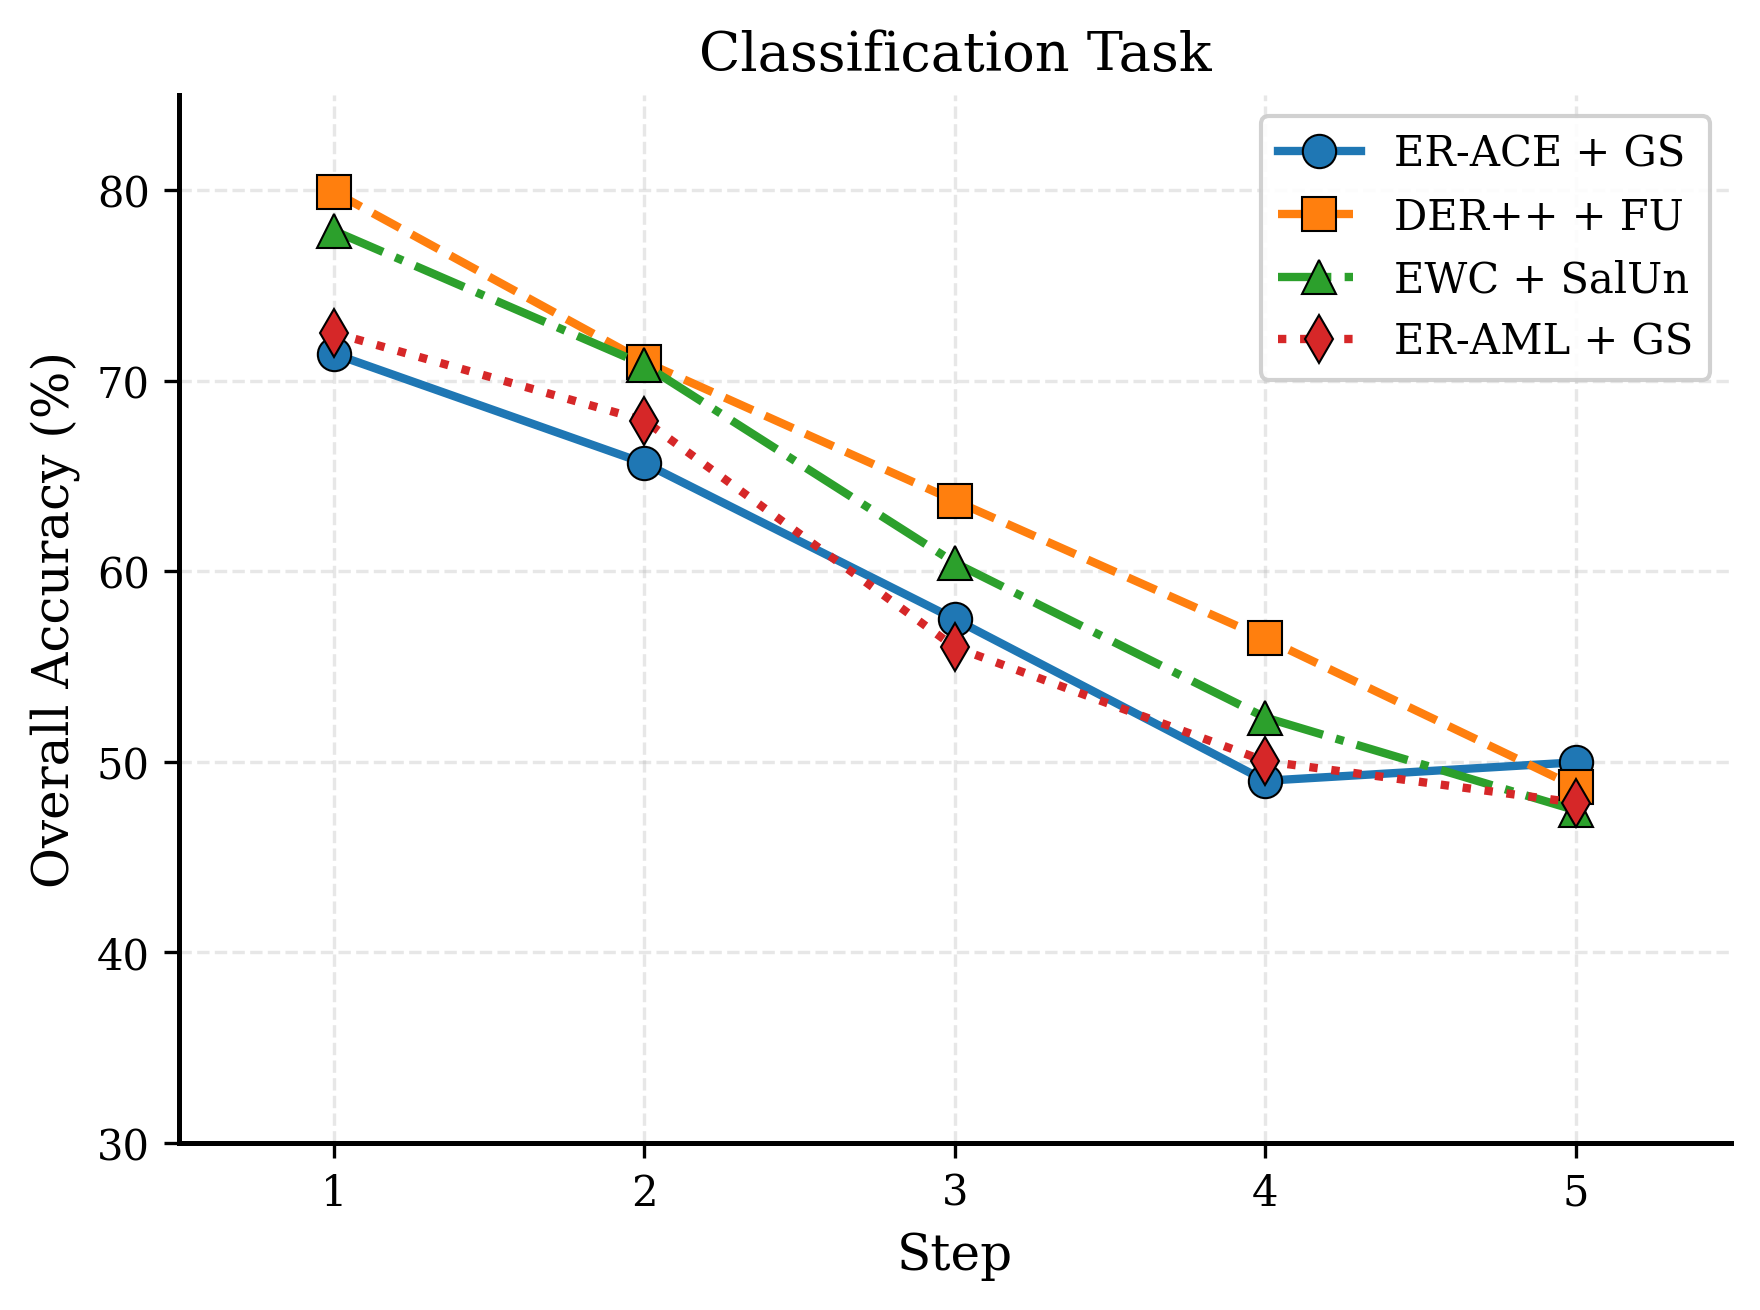
\includegraphics[width=\linewidth]{images/KL_classifaciton.png}
        \caption{CIFAR-100}
    \end{subfigure}
    \hspace{0.5em}
    \begin{subfigure}[b]{0.38\linewidth}
        \centering
        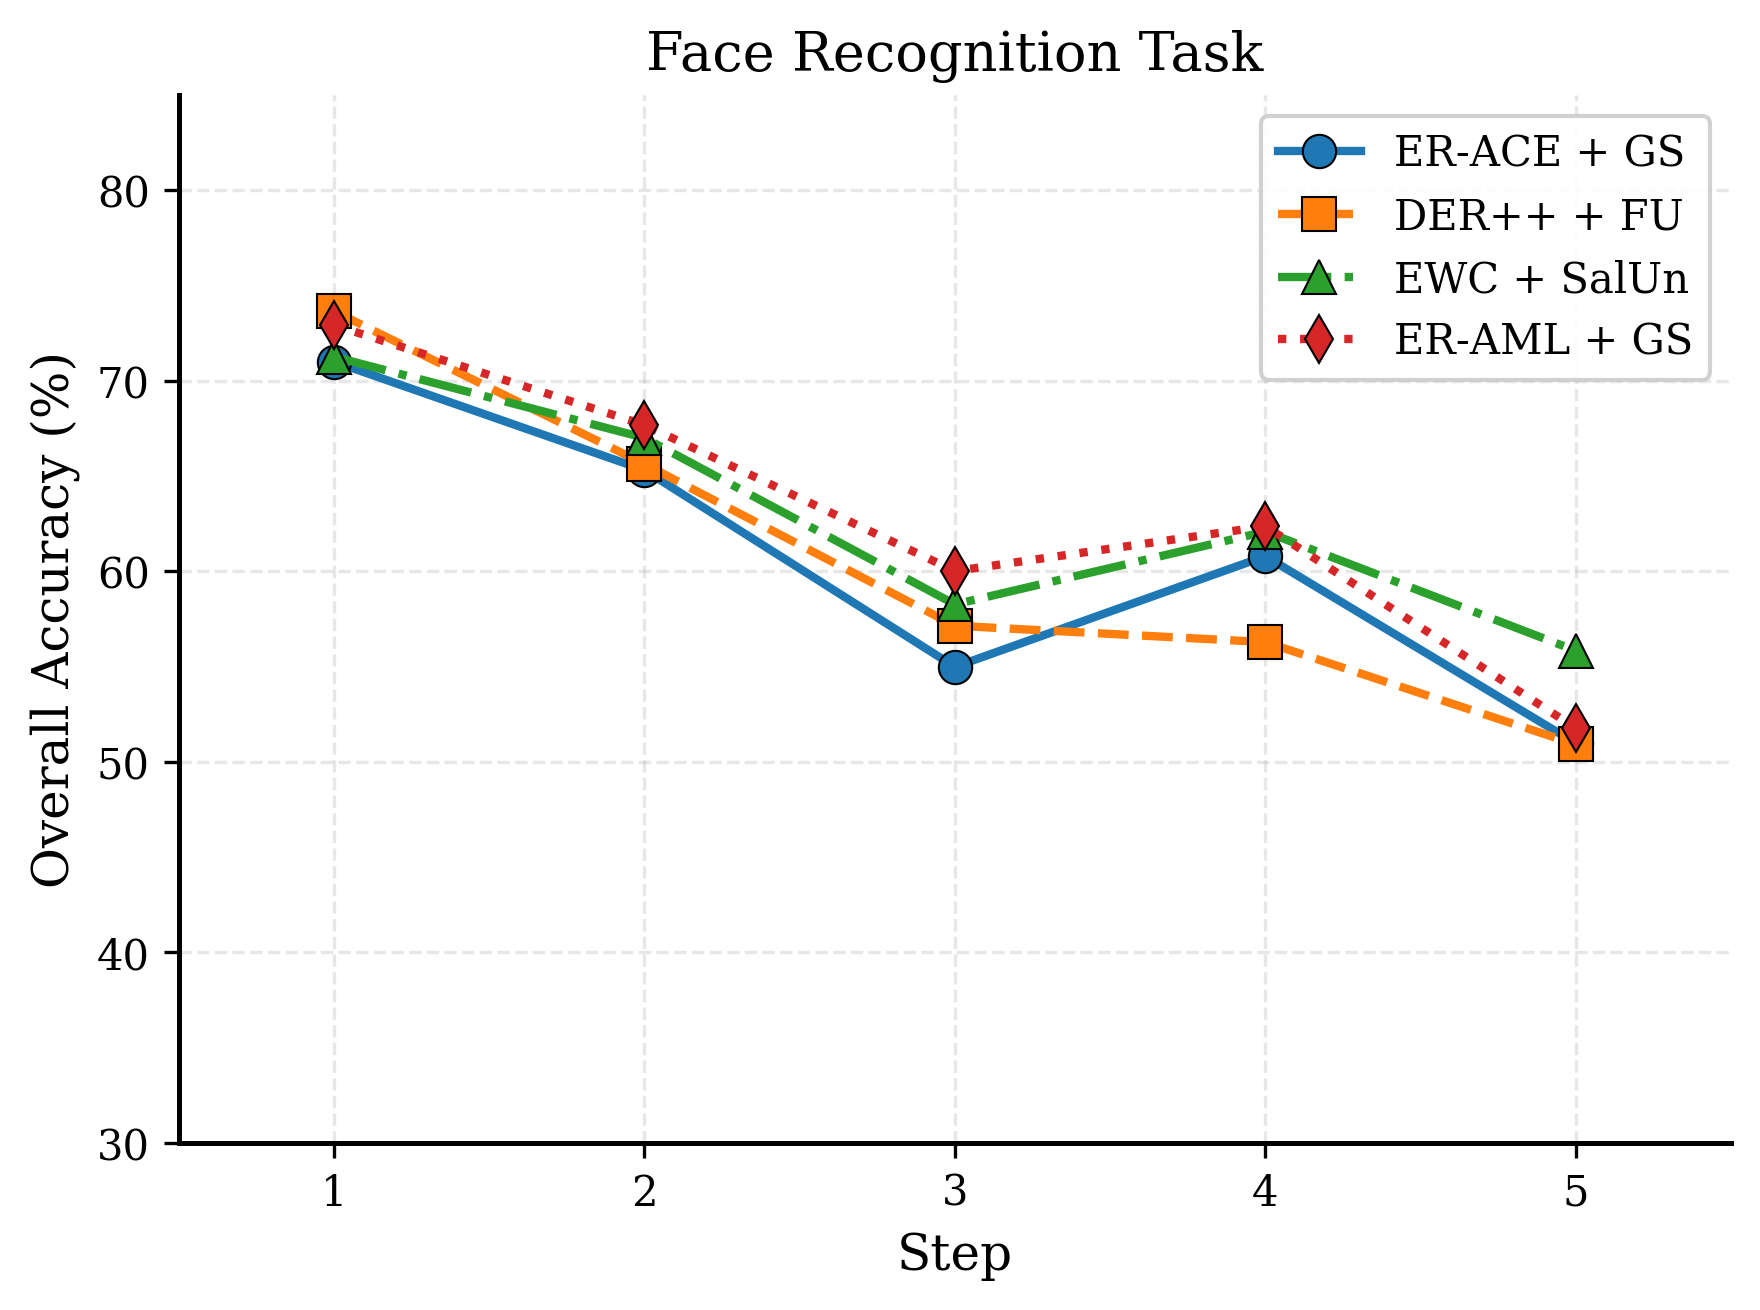
\includegraphics[width=\linewidth]{images/KL_face_Recognition.png}
        \caption{Face Recognition}
    \end{subfigure}
    \caption{Knowledge leakage in CL+MU combinations. Retain accuracy degrades progressively across CLU cycles on both benchmarks.}
    \label{fig:pilot_study}
\end{figure}

\section{Conclusion}
\label{6}
We introduced BID-LoRA, a parameter-efficient framework for Continual Learning and Unlearning (CLU) with three key contributions. First, Escape Unlearning pushes forget-class embeddings to a scaled escape point, enabling stable forgetting without disrupting retained knowledge. Second, dedicated adapters for retention, acquisition, and forgetting eliminate parameter interference and knowledge leakage. Third, the framework achieves competitive CLU performance with only $\approx$5\% tunable parameters, at a fraction of the cost of full fine-tuning. Experiments on CIFAR-100 and \textcolor{red}{VGGFace2} show BID-LoRA achieves the best or second-best overall accuracy in most tasks while consistently minimizing forget accuracy. Our sliding window protocol establishes \textcolor{red}{a benchmark, within the vision classification and face-recognition settings evaluated here,} for validating complete knowledge replacement over multiple CLU cycles, offering promising empirical evidence for real-world applications under privacy and regulatory constraints\textcolor{red}{, though these benchmark-level results do not constitute a formal or certified privacy guarantee (see Broader Impact Statement)}. Future work will eliminate retention buffers entirely, reducing them from 10\% to 0\%, and extend to other biometric modalities such as iris and fingerprint recognition, where privacy-driven unlearning is critical.
\section*{\textcolor{red}{Broader Impact Statement}}
\textcolor{red}{BID-LoRA's continual unlearning capability supports privacy compliance (e.g., GDPR/CCPA data-deletion requests) but is dual-use: the same enrollment/removal mechanism could extend surveillance or access-control systems, particularly given our face-recognition evaluation. Our empirical metrics (forget accuracy, MIA, KL divergence) demonstrate promising unlearning behavior but do not constitute a formal privacy guarantee; residual information may remain recoverable under stronger extraction, inversion, or adaptive attacks not evaluated here. Because face-recognition accuracy can vary across demographic groups, repeated learn-forget cycles may introduce or amplify subgroup disparities, warranting fairness audits. Finally, the retain-data replay buffer requires governance -- its storage, access, and retention policies should be scrutinized to avoid becoming a new privacy risk.}


\bibliography{tmlr}
\bibliographystyle{tmlr}

\appendix
% \section{Appendix}
% Add appendix content here if needed.

\end{document}
